% document.tex
% 请使用最新发行版本的TeX Live编译(编译方式为XeLaTeX)。
\documentclass[master,academic]{ysuthesis} % Use the custom document class
%%%%%%%%%%%%%%%%%%%%%%%%%%%%%%%%%%%%%%%%%%%%%%%%%%%%%%%%%%%%%%%%
%	博士/硕士
%	doctor——博士,中英文对照的图题和表题采用命令\bicaption{中文标题}{英文标题}实现,子图使用命令\bisubcaptionbox{中文标题}{英文标题}[]{}实现。
%	master——硕士(默认选项),中文的图题和表题采用用命令\caption{标题}实现,子图使用命令\subcaptionbox{中文标题}[]{}实现。
%%%%%%%%%%%%%%%%%%%%%%%%%%%%%%%%%%%%%%%%%%%%%%%%%%%%%%%%%%%%%%%%
%   学术学位/专业学位
%	academic——学术学位(默认选项)
%	professional——专业学位
%%%%%%%%%%%%%%%%%%%%%%%%%%%%%%%%%%%%%%%%%%%%%%%%%%%%%%%%%%%%%%%%

%%%%%%%%%%%%%%%%%%%%%%%%%%%%%%%%%%%%%%%%%%%%%%%%%%%%%%%%%%%%%%%%
%	图片路径
\graphicspath{{fig/}}
%%%%%%%%%%%%%%%%%%%%%%%%%%%%%%%%%%%%%%%%%%%%%%%%%%%%%%%%%%%%%%%%

%%%%%%%%%%%%%%%%%%%%%%%%%%%%%%%%%%%%%%%%%%%%%%%%%%%%%%%%%%%%%%%%
%	Document metadata
%%%%%%%%%%%%%%%%%%%%%%%%%%%%%%%%%%%%%%%%%%%%%%%%%%%%%%%%%%%%%%%%
\title{生物同步康复机制理论与应用}{Bio-Syncretic Rehabilitation Mechanism Theory and	Application}
\author{张小明}{Zhang Xiaoming}
\school{电气工程学院}{School of Electrical Engineering}
\subject{电气工程}{Electrical Engineering}
\applydegree{工学}{Engineering}
\supervisor{郭大师}{教授}{Guo Dashi}{Professor}
\assosupervisor{吴高工}{高级工程师}{Wu Gaogong}{Senior Engineer}
\date{2024年6月}{June, 2024}
\bookclassificationnumber{TM464}{621.3}
\security{公开}
\researchtype{产品研发}%产品研发、应用研究、工程设计、基础研究等,学术学位可忽略

%packages
\usepackage{algorithm}
\usepackage{algorithmic}

\begin{document}

	\makecover

	\cabstract{}

	\ckeywords{关键词1;关键词2;……;关键词8}

	\eabstract{The rehabilitation mechanism is the foundation for a rehabilitation robot to realize its motion, and the quality of the rehabilitation mechanism decides the rehabilitation effect of patients with the rehabilitation robot. The research of rehabilitation mechanism is the key content in rehabilitation engineering. The bio-syncretic rehabilitation mechanism (BSRM) is a new type of modern mechanism composed of human body and machine, and it can meet the design requirements of rehabilitation robot more effectively because of the interaction and harmonization between human body and machine during the rehabilitation exercise. This paper presents the relative systematic research on BSRM and its application. The main contents of this paper are as follows:

		The concept of rehabilitation mechanism is proposed based on the relationship between human body mechanism and mechanical mechanism in the rehabilitation kinematics system, and the characteristics, degree of freedom, classification and symbol representation of this new kind of mechanism is introduced. The approaches to type synthesis of parallel BSRM and series BSRM are developed based on screw theory and the characteristic of BSRM, and some parallel BSRMs for ankle joint rehabilitation and series BSRMs for knee joint rehabilitation are got.
	}

	\ekeywords{keyword1; keyword2; ……; keyword8}

	\customizedtableofcontents

	\chapter{绪论}
	\section{研究背景与意义}
	随着科技的不断进步与社会对智能化技术需求的增加,自动驾驶技术在多个领域得到了广泛应用。从无人驾驶汽车到无人驾驶清扫车,智能化交通工具逐步融入日常生活中,改变了传统的交通方式,提高了工作效率,保障了安全性。无人驾驶技术的快速发展为城市环卫、仓储物流等多个领域提供了新的解决方案,尤其是在复杂环境中的智能作业能力,使得人力资源的需求大幅减少,降低了事故发生的概率,推动了社会的可持续发展。
	铰接车作为一种具有独特结构的车辆,其在车辆动力学和控制领域具有较高的研究价值。不同于常规车辆,铰接车通过中间铰接部分实现转向,具有较强的灵活性和转弯能力,但也因此带来了更复杂的运动学约束和控制问题。铰接车的运动规划涉及到如何高效、安全地控制其在复杂环境中的行驶轨迹,特别是在低速、精确行驶的应用场景中,如何确保车辆能够稳定执行任务,同时避免与环境中的障碍物发生碰撞,是研究的核心问题。
	近年来,铰接车的应用逐渐扩展至仓储搬运、城市环卫等多个领域。在环卫作业中,铰接车具有较高的机动性和灵活性,能够应对复杂的城市道路环境,尤其是在狭窄的街道和交通繁忙的区域,铰接车凭借其独特的转向方式能够完成更为精细的作业任务。因此,研究铰接车的运动规划技术,尤其是在复杂环境下的路径规划与速度控制,具有重要的现实意义。
	本课题旨在研究铰接车在不同应用场景下的运动规划问题,重点探索如何在存在障碍物、复杂地形和环境变化的情况下,设计高效的运动规划算法。通过分析铰接车的运动学模型,结合车辆的工作环境和任务要求,本文将设计适应铰接车特性的轨迹生成与速度规划方法,以提升铰接车的运动性能,保证其在实际应用中的高效性、安全性与稳定性。
	铰接车作为一种具有独特结构和控制需求的车辆,其运动规划技术的研究不仅能够提升其在各种复杂环境中的应用能力,也为智能交通和自动化系统的进一步发展提供了技术支撑和理论基础。
	\section{运动规划技术国内外研究现状}
		\subsection{基于图搜索的运动规划方法}
		路径规划算法的演进历程始终围绕环境复杂性、计算效率与最优性之间的权衡展开。早期研究聚焦静态结构化环境中的最优路径求解:Dijkstra算法(1959)通过广度优先策略首次系统化解决带权图的最短路径问题,但其盲目搜索特性导致时间复杂度高达$O(n²)$,难以应用于大规模场景。Hart等人(1968)提出的A算法创新性地引入启发式函数$h(n)$,将搜索方向引导至目标节点,在保证路径最优性的前提下将复杂度降低至$O(b^d)$(b为分支因子,d为搜索深度),奠定了启发式搜索的理论基础。然而,经典A算法仍面临两个关键限制:一是内存占用随搜索空间指数增长,二是启发函数设计依赖先验环境知识,难以应对动态障碍物或未知地形。

		动态环境下的增量式搜索技术突破解决了部分实时重规划难题。Stentz的D算法(1994)采用反向搜索机制与增量更新策略,仅在环境变化时局部修正路径,将重规划耗时从O(n²)降至O(k)(k为变化区域节点数),使机器人能在未知地形中实时避障。但D算法仍存在路径振荡问题,且在复杂动态场景中频繁更新导致累积误差。Koenig等人提出的LPA*(2004)通过维护优先队列的键值一致性,实现历史搜索信息的智能复用,使得连续规划场景的搜索速度提升40%以上,但其内存管理机制仍无法有效应对长期运行中的状态爆炸问题。Likhachev团队同期提出的AD与ARA算法(2003-2004)引入次优性容忍系数,允许算法在有限时间内输出渐进优化的路径,为实时性要求严苛的无人机导航提供了解决方案,但路径质量与计算速度的定量关系仍需人工调参,缺乏自适应能力。

		实时响应与高维空间规划的需求推动了算法框架的革新。Bulitko的LRTS(2004-2011)通过剪枝冗余状态与动态调整搜索深度,将实时启发式搜索的响应延迟控制在毫秒级,但其剪枝策略可能丢失潜在最优路径。Harabor的JPS算法(2011)针对栅格地图提出"跳跃点"理论,通过识别路径对称性跳过大量无效节点,在保持最优性的前提下将搜索速度提升10倍以上,但该方法仅适用于均匀网格环境,且无法处理动态障碍物。Koenig与Likhachev的RTAA*(2012)结合在线学习机制,利用实际移动代价动态更新启发函数,使智能体在未知地形中的路径收敛速度提升60%,但其学习过程需要大量交互数据,在稀疏奖励场景中表现受限。

		当前研究面临的核心挑战集中于多维矛盾的协同优化:① ​高维状态空间的可扩展性:现有算法在3D无人机路径规划或机械臂关节空间规划中,因维度灾难导致计算复杂度激增;② ​动态不确定性的鲁棒性:多数算法假设环境变化可感知且离散,但在实际应用中(如人群密集区域),障碍物运动预测误差与传感器噪声可能引发路径失效;③ ​多目标协同规划:自动驾驶场景中需同时优化路径长度、安全性、能耗等多目标,传统单目标优化框架难以满足;④ ​在线学习与先验知识的融合:尽管深度强化学习(DRL)在复杂环境规划中展现出潜力,但其黑箱特性与高样本复杂度制约了工业部署。近期研究尝试通过分层规划(如RRT与A的混合架构)、元启发式优化(如NSGA-II多目标遗传算法)以及神经启发函数学习(如将CNN集成至A*的h(n)估计)等方式突破瓶颈,但理论完备性与工程实用性之间仍存在显著差距。
		\subsection{基于采样的运动规划方法}
		路径规划算法的研究在20世纪末迎来转折点,LaValle(1998)提出的Rapidly-exploring Random Trees (RRT)​ 首次将随机采样与树形结构结合,通过偏向未探索区域的生长策略有效应对高维构型空间和非完整约束问题。RRT的概率完备性​(即随着样本数增加,找到可行解的概率趋近于1)奠定了采样算法的理论基础,但其生成的路径质量(如长度、平滑度)无法保证最优。随后,Kuffner与LaValle(2000)提出RRT-Connect,通过双向树生长与贪心连接策略(CONNECT启发式)显著提升单次查询效率,解决了传统RRT在复杂环境中收敛速度慢的问题,成为实时机器人导航的重要工具。然而,这一阶段的算法仍局限于可行解搜索,缺乏对路径最优性的理论保证。
		针对动态环境下的实时规划需求,Bruce与Veloso(2001)提出Execution-extended RRT (ERRT),引入路径点缓存(Waypoint Cache)和自适应成本惩罚机制,在重规划中复用历史路径信息,解决了传统RRT在动态障碍物场景下的重复计算问题,首次实现了机器人系统的实时在线规划。然而,ERRT的路径优化依赖启发式规则,缺乏全局最优性保证。同期,Gammell等人(2010)的Informed RRT​ 通过椭圆启发式采样(Ellipsoidal Heuristic)将搜索空间限制在可能改进当前解的椭圆区域内,显著提升收敛速度与最终路径质量,首次在理论上证明采样算法可渐进趋近最优解。这一工作揭示了传统RRT因全局均匀采样导致的效率瓶颈,为后续最优性导向算法奠定了基础。
		2011年成为路径规划算法发展的分水岭。Karaman与Frazzoli的里程碑工作PRM与RRT​ 严格证明了传统PRM和RRT无法保证渐进最优性(即解的成本不收敛至理论最小值),并提出基于动态邻域半径的改进算法。PRM通过自适应调整连接半径(与样本数成反比),确保概率完备性与渐进最优性;RRT则引入代价敏感的树重布线机制,在保持单次查询效率的同时实现解质量的单调提升。同年,Gammell等人的**Batch Informed Trees (BIT*)**​ 融合图搜索(A*启发式)与批处理采样,在隐式随机几何图(RGG)上执行增量搜索,解决了高维空间(如14自由度机械臂)中传统算法收敛缓慢的问题。这些工作标志着采样算法从“可行解搜索”迈入“最优解保证”的新阶段,但其计算复杂度与高维场景的适应性仍面临挑战。尽管上述算法在理论与应用上取得显著进展,仍存在以下关键挑战:
		​高维扩展性:RRT*等算法在高维空间(如>8维)中因邻域查询与重布线开销剧增,难以满足实时需求。
		​动态环境适应性:现有方法(如ERRT)依赖历史路径缓存,对突发障碍物或快速变化场景的鲁棒性不足。
		​理论分析局限:多数渐进最优性证明假设环境为凸集或无障碍,复杂非凸环境下的收敛速率与采样策略仍需深入探讨。
		​多目标权衡:路径长度、安全性、能量消耗等多目标优化尚未被系统整合,启发式规则设计缺乏理论指导。

		\subsection{基于曲线插值的运动规划方法}
		路径规划作为自主导航系统的核心技术,经历了从基础几何方法到复杂优化算法的演进过程。早期研究多集中于静态环境下的几何路径求解,1990年Reeds和Shepp的开创性工作《Optimal paths for a car that goes both forwards and backwards》奠定了车辆运动规划的理论基础。该研究在Dubins曲线基础上引入倒车机制,证明了包含至多两个尖点的CCSCC型路径(圆-圆-直线-圆-圆)即可构成最优解。通过构建48种候选路径形式,解决了双向行驶车辆在最小转弯半径约束下的最短路径问题。但该方法局限于二维平面几何推导,未考虑动态障碍物和实时计算需求,且候选路径的枚举式搜索在复杂场景下计算效率较低。 随着自动驾驶技术的发展,2017年百度Apollo团队在《Baidu Apollo EM Motion Planner》中提出分层运动规划框架,标志着路径规划开始向动态环境适应性和多约束协同优化方向演进。该系统采用Frenet坐标系下的路径-速度迭代优化,结合动态规划粗搜索与二次规划细优化,首次实现了交通规则、障碍物决策与运动平滑性的多目标协同。其创新性地将决策问题转化为可行轨迹生成,通过构建凸可行空间保障解的存在性。但该方法依赖人工规则进行障碍物交互决策,在密集动态场景下存在策略僵化风险,且未充分考虑三维空间约束。 2018年Gao等人的研究《Online Safe Trajectory Generation For Quadrotors Using Fast Marching Method and Bernstein Basis Polynomial》推动了无人机领域的实时规划进展。该方法创新性地将快速行进法(FMM)与ESDF距离场结合,构建速度自适应的时空索引路径,解决了传统方法时间分配不合理的痛点。通过贝塞尔曲线的凸包特性,首次实现了轨迹整体安全性和高阶动力学约束的严格保证。实验证明其能在未知环境中实时生成安全轨迹,但飞行走廊膨胀策略在狭窄空间可能过于保守,且未有效处理动态障碍物的预测与避让。 2019年Nguyen团队在《Navigation with polytopes and B-spline path planner》中提出多面体导航工具箱,将路径规划抽象为凸多面体序列内的B样条优化问题。通过将B样条转换为等效贝塞尔表示,显著提升了局部凸性约束的紧密度,使线性约束控制点即可保证全局安全性。该工作构建了从栅格地图到多面体地图的完整流程,支持最小控制点、代数解等多种优化模式。但多面体序列的构建依赖静态环境假设,在动态场景中需要频繁重规划,且高维凸优化问题的实时性仍有提升空间。

		\subsection{基于优化的运动规划方法}
		2015年Li等人(文档1)首次提出基于时间最优控制的动态优化框架,将平行、垂直等规则停车场景与不规则障碍物场景统一建模。该方法严格描述车辆运动学、机械约束与碰撞条件,通过内点法求解非线性优化问题,突破了传统几何法仅处理特定场景的局限。其创新性在于构建了开放框架,允许用户自定义约束与优化目标。但缺陷在于未考虑不确定性环境,且计算复杂度高,难以满足实时性需求。同年,Kondak等(文档3)提出将路径规划转化为非线性最优控制问题,利用序列二次规划(SQP)直接优化轨迹,引入人工势场处理障碍物碰撞,支持全维车辆模型。然而,其势场函数设计依赖经验参数,且未解决非凸优化对初值敏感的问题。 
		2017年Arantes等(文档2)针对离散时间步间的“跳跃碰撞”问题,提出基于混合整数线性规划(MILP)的连续时间碰撞避免编码。通过约束相邻状态位于障碍物同侧,确保轨迹段安全性,并将机会约束引入风险分配框架,平衡路径安全性与保守性。该方法显著提升了非凸环境下的路径安全性,但MILP的NP-hard特性限制了其扩展性,难以应对大规模障碍物场景。2018年Zhang与Borrelli(文档5)进一步提出基于强对偶定理的平滑碰撞约束重构,将非凸避障条件转化为可微优化问题,支持全维物体与复杂障碍物,并通过符号距离函数量化侵入程度,实现“最小侵入”轨迹生成。但障碍物需分解为凸集,预处理成本较高。
		2020年Zhang等(文档5扩展研究)提出分层优化框架H-OBCA(文档4),融合混合A的全局搜索与优化碰撞避免(OBCA)的局部精细化。混合A基于简化模型快速生成粗路径,OBCA利用全维模型优化平滑性与动态可行性,解决了非凸优化依赖初值的瓶颈。实验表明其在狭窄场景中可实现实时规划(<1s),且轨迹可被底层控制器精准跟踪。然而,其性能受限于混合A*的路径质量,复杂障碍布局下可能陷入局部最优。2021年同团队(文档4)进一步引入时间变量优化与自适应风险分配,提升算法对动态障碍的鲁棒性,但多车协同场景下的博弈行为仍未解决。

	\section{铰接车运动规划技术国内外研究现状}
	铰接车路径规划的研究历程可追溯至2010年代初期的几何建模与静态环境规划阶段。早期的代表性工作如Choi与Huhtala(2015)提出基于Bézier曲线的分层规划框架,其核心贡献在于将参数化曲线与搜索算法结合,通过离线生成满足非完整约束的运动基元库(包含曲率连续的前进/倒车路径片段),再结合A*算法在线搜索全局路径,并引入非线性优化修正关节角度超限问题。该方法在港口AGV实验中成功将路径规划耗时降低37%,且路径成功率提升至92%(测试场景为90°直角弯道,铰接角限制±45°),但受限于Bézier曲线的曲率连续性仅达G2级别,导致跟踪时仍需额外的速度平滑处理,且未考虑动态障碍物避让。紧随其后的Sarata团队(2016)针对轮式装载机的V型作业路径提出对称Clothoid曲线连接策略,通过数学证明得出Clothoid曲线的曲率线性变化特性可消除传统线-弧路径的曲率突变问题,实验数据显示转向角波动幅度减少58%(测试机型:沃尔沃L220G装载机),但其固定路径模式依赖预设的装载点与卸载点位置,难以适应砂石堆形状动态变化的非结构化场景。 随着实时计算能力的提升,2010年代中后期研究重点转向动力学模型集成与在线优化算法。Nayl等(2017)首次将模型预测控制(MPC)与Bug算法结合,提出基于铰接车误差动力学模型的滚动优化框架,通过实时调整前轮转向角与车速实现动态避障。该方法在仿真中成功处理了突然出现的移动障碍物(最大速度2m/s),路径跟踪误差控制在±0.15m以内,但未解决多周期任务的长时优化问题,且在狭窄通道中易因局部最优陷入死锁。Chen等(2018)系统对比了简化单车模型与双体铰接模型的规划效果,发现复杂模型在双向倒车场景中可生成更短的安全路径(平均缩短19%),但计算耗时增加75%,揭示了模型精度与实时性之间的固有矛盾。Hong团队(2020)进一步引入3D地形高程数据构建动力约束,提出动态规划(DP)与MPC结合的混合方法,在轮式装载机的崎岖地形实验中实现能耗降低22%(测试地形坡度≤15°,摩擦系数0.4-0.6),但其离散化状态变量导致高维空间下的计算复杂度呈指数级增长,难以扩展至多关节车辆。 近年来,研究焦点转向多目标协同优化与数据驱动方法。Kawabe等(2021)设计的分级优化框架将全局任务分解为铲取点选择、卸载点规划与局部路径生成子问题,并首次引入深度强化学习(DRL)实现动态砂石堆的自适应装载路径规划。该方法在仿真中完成分布式砂石堆的全转移任务(堆数≤5,间距≥3m),效率较传统人工规则提升41%,但仿真与实车的传感器噪声差异导致迁移后定位误差放大至0.3m以上。Zhao等(2023)采用Chebyshev伪谱法对重型铰接车垂直泊车问题进行时间最优轨迹优化,通过精确建模非完整约束与防折叠(anti-jackknife)限制,在2.5m宽窄道场景中生成无碰撞路径的成功率达98%,平均规划时间仅需0.8秒(对比传统RRT*算法的12秒),但未考虑液压执行器的200ms延迟特性,实车测试中末端姿态偏差达±8°。Shi团队(2023)提出的自适应MPC跟踪系统通过曲率扰动补偿机制,在非均匀路面下将路径跟踪的横向位移误差降低65.7%(实测数据:误差从0.25m降至0.08m),但其依赖RTK-GPS的高精度定位信号,在卫星遮挡的室内仓储场景中性能显著下降。   
	现存挑战:尽管上述研究取得显著进展,铰接车路径规划仍面临动态环境适应性不足(如突发障碍物响应延迟>1.5秒)、计算效率瓶颈(复杂模型单次规划耗时>100ms)、多目标优化缺乏量化权衡准则(安全、能耗、时间的帕累托前沿尚未明确)等核心难题。此外,学习型方法的仿真到实车迁移性能衰减(平均效率损失≥30%)、极端工况(坡度>25°或摩擦系数<0.3)下的稳定性控制、多车协同冲突消解等方向仍需突破。未来研究或需融合轻量化神经网络加速优化计算、不确定性量化(UQ)增强鲁棒性,以及车-路协同感知框架,以实现矿山、港口等复杂场景的全天候自主作业。

	\section{本文研究目标和主要内容}
	本研究针对无人铰接车辆在复杂非结构化环境中的轨迹规划问题,提出一种融合全局与局部规划的优化框架,旨在解决传统路径规划算法因忽略铰接车强非完整性与运动学约束导致的路径不可跟踪、避障安全性不足等核心问题。

	本课题的研究内容如下:
	(1)基于优化的轨迹规划问题建模

	(2)基于微分平坦全局轨迹规划方法
	建立铰接车低速运动学模型,推导前后桥位姿变换关系与状态方程,证明其微分平坦特性,以平坦输出变量(前轴中点坐标)表征系统状态。给出平坦输出变量与航向角、铰接角、速度等状态量的解析表达式,为轨迹参数化提供理论支撑。采用Minco样条(Minimum Control Effort Spline)对轨迹进行分段多项式参数化,通过BIVP(Boundary-Value Problem)闭式解保证轨迹的平滑性与低控制能量消耗。设计曲率约束松弛函数与安全走廊约束,将路径规划问题转化为无约束优化问题,利用L-BFGS算法高效求解,确保轨迹满足最大转向半径与避障要求。提出航点切向一致性约束与换向点处理机制,解决铰接车在多阶段任务中因航点切换导致的运动方向突变问题。结合RRT-Connect算法生成初始路径,通过安全走廊优化生成全局可行轨迹,适用于码头装卸、矿山运输等长距离多任务场景。

	(3)基于NMPC和安全走廊的铰接车轨迹规划研究
	将车辆几何简化为前后桥矩形组合模型,基于Bresenham算法实现栅格地图中的快速碰撞检测,支持动态障碍物避让。提出基于静态转向模型的节点拓展策略,以固定路径步长Δs替代传统时间离散化方法,降低搜索空间维度。设计铰接角变化率惩罚项与Reeds-Shepp曲线引导机制,提升搜索效率与路径质量。构建最优控制问题,以舒适性(加加速度)、能耗(铰接角速度)与时间为优化目标,引入高阶运动学约束(速度、加速度连续性)。通过安全走廊约束松弛函数与Sigmoid时间变量映射,将硬约束转化为软惩罚项,利用IPOPT求解器实现复杂约束下的高效优化。在仿真环境中验证全局与局部规划方法在动态障碍物、狭窄通道等场景下的有效性,对比传统算法(A*、RRT*)在路径曲率、避障成功率等指标的优越性。

	本课题主要解决的关键问题和创新点如下:  
	(1)将微分平坦理论引入铰接车轨迹规划,简化高维状态空间,提升优化效率。
	(2)全局规划中融合Minco样条与凸多边形安全走廊,局部规划中结合NMPC与动态避障,实现全维度安全保障。
	(3)通过路径步长离散化与铰接角突变惩罚机制,显著提升铰接车在复杂场景下的搜索效率与路径可行性。

	\section{本文结构安排}
	本文的结构安排和各章的内容如下:

	第一章:绪论。本章节主要阐述无人铰接车在复杂环境(如港口、矿山)中的运动规划研究背景与意义,分析铰接车非完整约束带来的轨迹规划挑战。系统梳理国内外运动规划技术的研究现状,包括基于图搜索、采样、曲线插值与优化的方法,以及铰接车专用算法的进展与局限性。最后,明确本文研究目标与创新点,提出融合全局与局部规划的优化框架,并概述全文的章节安排。

	第二章:无人铰接车运动规划系统方案设计​。本章节基于最优控制理论构建铰接车轨迹规划的数学模型,推导其运动学方程与状态约束(如曲率、避障)。阐述最优控制问题的求解方法,包括动态规划与模型预测控制(MPC)的结合策略,并将问题离散化为非线性规划形式。通过分析初始路径生成对求解效率的影响,提出分层优化框架(全局粗规划+局部精细化),为后续章节提供理论支撑。

	第三章:无人铰接车微分平坦全局轨迹规划方法​。本章节提出改进的全局规划算法:基于铰接车微分平坦特性,以Minco样条参数化轨迹,结合RRT-Connect生成初始路径;设计凸多边形安全走廊约束,通过松弛函数处理曲率与避障条件,利用L-BFGS算法实现高效优化。针对多阶段任务(如码头装卸),提出航点切向一致性约束与换向点处理机制,并通过仿真验证算法在复杂场景下的有效性。

	第四章:基于安全走廊的无人铰接车局部轨迹规划方法​。章节提出局部规划解决方案:改进Hybrid A*算法,引入路径步长离散化与铰接角突变惩罚机制,结合Reeds-Shepp曲线加速搜索;构建基于安全走廊的NMPC框架,以舒适性、能耗与时间为优化目标,集成精确碰撞检测算法(Bresenham栅格检测)与高阶运动学约束,通过IPOPT求解器实现动态避障与实时轨迹优化,并通过仿真对比验证算法性能。

	第五章:结论与展望​。本章节总结全文研究成果,包括微分平坦理论在铰接车规划中的应用、安全走廊约束的优化方法,以及全局-局部协同规划框架的有效性。同时指出当前研究的局限性(如动态障碍物预测不足、多车协同未涉及),提出未来改进方向:融合深度强化学习提升自适应能力,开发轻量化模型以降低计算开销,并扩展至多机协同与三维地形场景。

	\chapter{铰接车建模与运动规划系统设计}
	本章节将首先我们的运动规划系统框架,它包括有全局规划和局部规划两个部分。然后基于最优控制问题框架给出轨迹规划问题的求解方法。介绍外点法和内点法在优化问题中的使用。
	\section{运动规划系统总体方案设计}
	我们的运动规划系统采用全局-局部双级递进架构实现任务分解。在全局层面,规划过程解耦为路径搜索与轨迹优化两个阶段:首先基于RRT/A*/JPS等前沿搜索算法快速生成无碰撞粗解路径,随后通过基于能量最优代价构建优化模型,在保障路径连续性的同时实现平滑性提升与运动学上的可行性。局部规划层面向实时运动控制需求,提出改进型Hybrid A*算法生成满足车辆运动学约束的可行路径,进而构建速度剖面作为轨迹优化初值。最终通过非线性模型预测控制(NMPC)框架实施时空联合优化,其安全边界通过动态安全走廊技术进行在线更新,确保规划结果同时满足实时性要求与严格的安全准则。运动规划系统的总体方案如下:
		\begin{figure}[!ht]
			\centering
			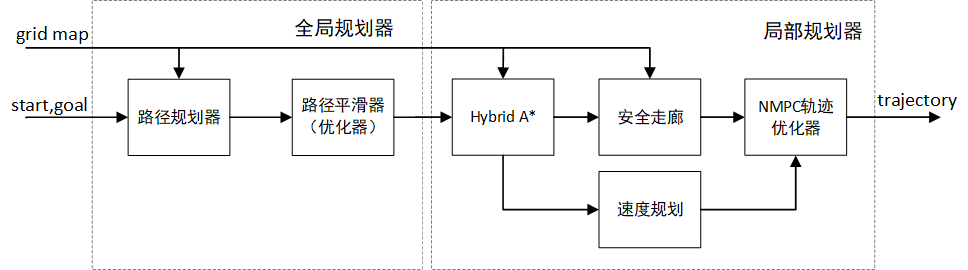
\includegraphics[width=1.0\textwidth]{运动规划算法框架.png}
			\caption{运动规划算法框架}
			\label{fig:运动规划算法框架}
		\end{figure}

	\section{铰接车运动学模型建立}
	铰接车总体上一共由前桥和后桥组成,中间通过液压或者舵机驱动铰接角完成转向。本文介绍的铰接车结构模型如下:  
	%图片  
	\begin{figure}[!ht]
		\centering
		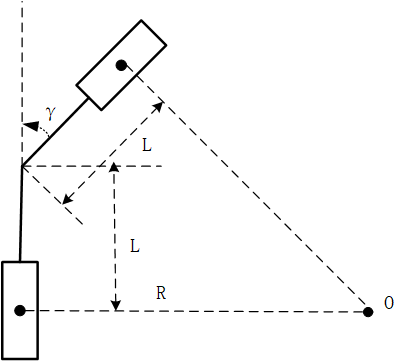
\includegraphics[width=0.6\textwidth]{铰接车简易模型.png}
		\caption{铰接车简易模型}
		\label{fig:铰接车简易模型}
	\end{figure}
	如上图所示,我们假设前轴中点作为参考点,前轴的航向角为theta1,后轴航向角为theta2。其中o点为瞬时转向圆心,pf为前轴中点pr为后轴中点,lf是前轴长度,lr是后轴长度,gamma是铰接角。为了推出铰接车的运动学模型,我们做出以下两个假设。(1)铰接车辆始终保持低速运动,忽略动力学特性。(2)假设车辆不发生侧滑。
	首先由于车辆不会发生打滑,所以车辆运动时前后车轮完全满足车辆的滚动约束,即速度方向和车辆的朝向保持一致。得到以下方程:
	\begin{equation}
		\begin{aligned}
			&\dot{x}_1=vcos\theta _1\\
			&\dot{y}_1=vsin\theta _1\\
			&\dot{x}_1sin\theta _1-\dot{y}_1cos\theta _1=0\\
			&\dot{x}_2sin\theta _2-\dot{y}_2cos\theta _2=0
		\end{aligned}
	\end{equation}
	由于前桥和后桥通过铰接角刚性连接,我们可以推导出前桥参考点和后桥参考点的坐标变换公式如下:
	\begin{equation}
		\begin{aligned}
			&x_1=x_2+l_2cos\theta _2+l_1cos\theta _1\\
			&y_1=y_2+l_2sin\theta _2+l_1sin\theta _1\\
			&\theta _2=\theta _1-\gamma 
		\end{aligned}
	\end{equation}
	以前桥为参考点,定义$(x,y,theta,gamma)$为铰接车的位姿,他们分别代表着$x_f,y_f,\theta_1,\gamma$。在我们的研究中铰接车的前桥和后桥相等,即$lf=lr=L=1.3m$。联合上式我们可以得到铰接车的运动学方程为:
	\begin{equation}
		\begin{aligned}
			\frac{d}{dt}\left[ \begin{array}{c}
				x_f\\
				y_f\\
				\theta\\
				\gamma\\
			\end{array} \right] =\left[ \begin{array}{c}
				vcos\theta\\
				vsin\theta\\
				vtan( \gamma /2 ) /L+\omega /( cos\gamma +1 )\\
				\omega\\
			\end{array} \right] 
		\end{aligned}
	\end{equation}
	其中$v,w$是输入量,分别代表这前轴速度和铰接角速度。
	其次我们可以推导出铰接车的转弯半径为:
	\begin{equation}
		\begin{aligned}
			R = \frac{v}{\theta} = v\cdot L \frac{1+cos\gamma}{vsin\gamma+L\omega }
		\end{aligned}
	\end{equation}
	特别的,日过我们忽略铰接车的动态转向,只保留静态转向,即$\omega=0$:
	\begin{equation}
		\begin{aligned}
			R_{steady} = \frac{L}{tan(\gamma/2)} 
		\end{aligned}
	\end{equation}

		
		
	\section{基于最优控制的运动规划问题建模}
	本文设计的全局和局部规划器都使用了基于优化的方法,将问题构建在最优控制的框架下求解。最优控制的一大特点就是可以清晰的把各种约束表示在问题里,例如运动学方程约束、状态受限约束和执行器受限约束,因此最优控制在轨迹规划中被广泛关注。假设系统状态方程为$\dot{x(t)}=f(x(t),u(t))$,最优控制就是从可选择的容许控制集$U$中,找到一个控制矢量$u(t)$,使得系统到终端时刻时,性能指标$J$取最小值,满足条件的控制成为最优控制$u^{*}(t)$,对应的状态方程的解成为最优轨线$x^{*}(t)$。最优控制侧重于得到系统的最优控制量,轨迹规划与之不同,它侧重于得到系统的状态量,即最优轨线。轨迹规划在最优控制的表述下属于代价函数是综合型或鲍尔扎型的性能指标,它通常包括能量消耗和终点代价两个部分。
	
	基于连续系统的鲍尔扎型最优控制可以将轨迹规划表述为如下:
	\begin{equation}
		\begin{aligned}
			\min_{x(t),u(t),t} &J = \Phi[x(t_f)]+\int_{t_0}^{t_f}L[x(t),u(t),t]dt\\
			s.t. \ \ \ &\dot{x} = f(x(t),u(t))\\
			&x_{min}\le x(t) \le x_{max},u_{min}\le u(t) \le u_{max},t \in{t_0,t_f}\\
			&x(t_0)=x_{start},x(t_f)=x_{goal},\\
			&h(x(t))\cap C_{occ}=\varnothing 
		\end{aligned}
	\end{equation}
	其中$t_f$是终端时刻,$\Phi[x(t_f)]$是终端代价,也就是对目标的偏差。$x(t)$和$u(t)$分别代表状态量和控制量,$L[x(t),u(t),t]$表示过程代价,在轨迹优化中可以是能量消耗,也就是对控制量的代价。
	
	对于离散系统,一般代价泛函可以表示为:
	\begin{equation}
		\begin{aligned}
			J = \Phi[x(N)]+\sum_{k=k_0}^{N-1}L[x(k),u(k),k]
		\end{aligned}
	\end{equation}

	$x(t)$和$u(t)$表示车辆的状态量和控制量,$J$是最优控制的目标函数。在约束中,$\dot{x(t)}=f(x(t),u(t))$是车辆的运动学方程,$x_{min}\le x(t) \le x_{max},u_{min}\le u(t) \le u_{max}$分别代表系统的状态受限和输入受限,$x(t_0)=x_{start},x(t_f)=x_{goal}$表示起点和终点约束。$h(x(t))\cap C_{occ}=\varnothing$表示车辆的避障约束。其中$C_{occ}$表示障碍物区域。下面将详细介绍铰接车轨迹规划中的各个组成部分。

	\section{最优控制问题的解法}
	最优控制问题的求解方法主要可分为两类。一类是​解析解法,基于变分法原理与极小值原理的经典分析方法。这类方法能够通过严格的数学推导获得控制律的显式解析解,具有理论完备性强的特点。然而其应用范围受限于问题复杂度——当系统动力学方程非线性程度加剧或路径约束增多时,解析解的推导将面临难以逾越的数学障碍,导致方法失效。另一类是​数值解法,采用离散化策略将连续最优控制问题转化为非线性规划问题求解。此类方法虽能处理复杂约束条件与非线性系统,但随着精度要求的提升(包括时间离散密度与状态量精度),会导致优化变量维度呈指数级增长。由此产生的计算复杂度将显著延长求解时间,严重影响控制系统的实时性表现。这两类方法呈现不同的特性,解析解法在简单场景中具有理论优势却缺乏工程适用性。而数值解法具广泛适应性但受制于“维度灾难”带来的计算瓶颈。
	\subsection{极小值原理}
	作为最优控制理论的基石之一,庞特里亚金于1956年建立的极小值原理突破了经典变分法的约束条件限制。该原理通过引入协态变量构建哈密顿函数体系,在容许控制域内寻找使哈密顿函数极小的最优控制序列。相较于传统变分法,其核心创新在于允许控制变量存在闭集约束,并能有效处理终端状态受限的边值问题。在工程实践中,该原理为航天器轨道转移、机器人轨迹规划等典型最优控制问题提供了严格的判据,但在强非线性系统中的应用常受限于两点边值问题的解析求解困难,这推动了后续数值方法的发展。
	
	\subsection{基于打靶法的数值求解}
	前文探讨的极值条件理论虽然为最优控制律的存在性提供了严格判据,但在实际应用中面临显著的计算瓶颈。当系统动力学呈现强非线性特征或存在多类路径约束时,基于庞特里亚金原理的解析求解往往难以实现。针对此类复杂场景,需要建立具有工程可实现性的数值优化策略。本节阐述的打靶法即通过离散化处理将连续最优控制问题转化为有限维参数优化问题,不仅保持了最优性条件,同时为应用成熟的数值优化算法(如序列二次规划、内点法等)奠定了基础。

	该方法的核心思想在于,将状态微分方程在时间域上离散为代数方程组,进而构造具有可计算结构的非线性规划模型。具体而言,打靶法对控制量进行离散化,状态量作为控制量的函数,将原问题转化为关于离散节点的控制量寻优过程。这种方法只优化控制变量,变量的维度一般不会很高,对于最优控制有很大的应用场景。但是对于轨迹规划他就显得不是那么的时候,因为它并不会直接获得系统的状态,系统的状态需要由优化后的控制输入根据运动学模型进行航迹推演。因此,打靶法更适合轨迹跟踪这一类控制问题。打靶法的优化问题如下:
	\begin{equation}
	\begin{aligned}
		\min_{u_0,...,u_N} & J(u_0,u_1,\ldots,u_N,x_1,x_2,\ldots,x_N) \\
		& x_{k+1}=x_k+f(x_k,u_k)\cdot \Delta t,\quad k=0,\ldots,N \\
		& x_{0}=x_{start}
	\end{aligned}
	\end{equation}
	如上式,打靶法只优化控制变量,所以代价函数中的状态量全部时关于控制量$u$的函数。若想获得轨迹,还需要将优化出来的控制变量$u_0,...,u_k$使用运动学方程$x_{k+1}=x_k+f(x_k,u_k)$递推得到。
	下一小节我将介绍一种更为直接的数值方法,它可以直接获得系统的状态,也就是轨迹。
	
	\subsection{基于配点法的数值求解}
	与打靶法不同,打靶法只离散控制量,而配点法通过离散控制量和状态量将连续最优控制问题转化为非线性规划问题(nonlinear programming problem,NLP),其数值鲁棒性在工程领域广受认可。由于直接将状态量纳入到优化变量,所以配点法相较于打靶法更适合用来做轨迹规划。这种方法在配置节点处要求满足动力学方程约束,配点之间使用多项式或者其他曲线进行差值。当配点较为密集时,配点之间也可以近似用直线连接。

	本次设计中我们使用配点法求解,所以我们先对连续最优控制问题进行离散化,离散化后可以表示如下:
	\begin{equation}
	\begin{aligned}
		\min_{x(t),u(t),t} &J = \Phi[x(N)]+\sum_{k=0}^{N-1}L[x(k),u(k),k]\\
			s.t. \ \ \ &x(k+1) = x(k)+ \Delta t \cdot f(x(k),u(k))\\
			&x_{min}\le x(k) \le x_{max},u_{min}\le u(k) \le u_{max},k \in{0,N-1}\\
			&x(0)=x_{start},x(N)=x_{goal},\\
			&h(x(k))\cap C_{occ}=\varnothing 
	\end{aligned}
	\end{equation}
	上述式子中约束条件依次为系统动力学约束、状态受限约束、输入受限约束、起点终点约束和路径约束(安全避障约束)。

	第三章和第四章中我们会分别针对全局规划和局部规划对【公式】设计各自的具体目标函数和约束形式,并使用非线性优化求解器进行求解。非线性优化求解器我们将在【下一节】中介绍。

	\section{非线性规划问题的求解}
	在上一节中我们把最优控制离散化为了一个非线性规划(NLP)问题,这个问题一般具有很强的非线性和非凸性。一般处理NLP问题的求解方法有很多,包含增广拉格朗日乘子法(ALM)、交叉方向乘子法(ADMM)、罚函数法、有效集法和可行方向法等。这些所有的方法都假设了问题和约束都是凸的,目前对于非凸问题还没有有效的求解方法。由于罚函数在工程中表现优异,在本设计中也将使用罚函数。
		\subsection{罚函数法}
		无约束问题的求解有梯度一类的方法和牛顿法一类的方法,这些方法被公认可以有效解决无约束优化问题。所以对于带约束的优化问题我们一般可以使用罚函数把它化为无约束优化问题。
		罚函数有内罚函数和外罚函数两种,其代表性求解器分别是IPOPT和G2O。考虑如下一般的优化问题:
		\begin{equation}
			\begin{aligned}
				\min_{x} &J(x)\\
					s.t. &g(x)<0\\
					&h(x)=0
			\end{aligned}
		\end{equation}
		公式【】中包含通用的两种约束,等式约束和不等式约束。我们可以直接把这两种约束使用罚函数加到代价函数中:
		\begin{equation}
			\begin{aligned}
				\min_{x} &J(x)+Pen1(g(x))+Pen2(h(x))
			\end{aligned}
		\end{equation}
		罚函数Pen1针对于处理不等式约束,它必须具有的特性是在可行域外时代价尽量大,在可行域内时代价尽量小。罚函数Pen2针对于处理等式约束,它必须具有的特性是在可行点外时代价尽量大,在可行点内时代价尽量小。在大多数时候,我们其实并不关心使用内罚还是外罚,我们更关心的是找到两个合适的罚函数来使得问题求解起来更加的鲁棒。
		\subsection{非线性规划问题的初始解}
		罚函数仅仅是将带约束的问题转化为了无约束优化问题,求解这么一个无约束优化问题还需要一个迭代初始解。在凸优化中,迭代初始解我们是很关心它的质量,凸特性会使得初始解迫向最优解迭代,初始解的不同只是影响收敛快慢而已。但是在我们的非线性规划问题中,问题是强非凸的,所以不同的初始解可能最终收敛到的极值并不一样。所以找到一个优秀的初始解往往可以使得最终的求解结果接近最优解。
		\begin{figure}[!ht]
			\centering
			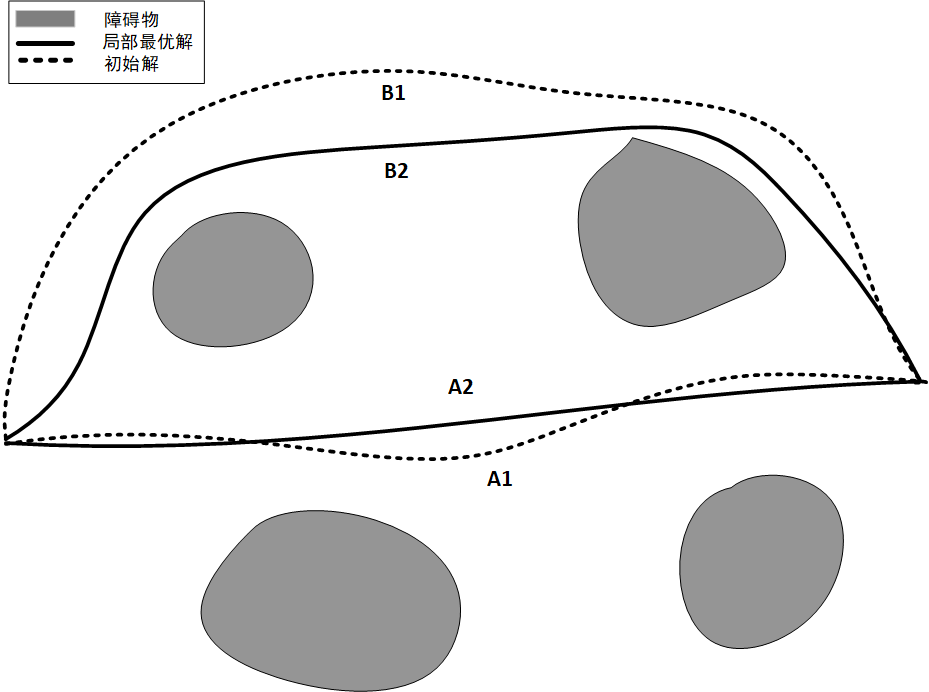
\includegraphics[width=0.8\textwidth]{不同初解.png}
			\caption{不同初解}
			\label{fig:不同初解}
		\end{figure}
		如图【】所示,非线性规划算法处理初始轨迹A1后将迭代优化至轨迹A2,而选取初始方案B1时则会收敛于轨迹B2。通过图示对比可明显观察到,采用初始轨迹A1能使系统收敛至路径长度更优的局部极小值。该现象验证了初始参数设定对优化结果具有决定性作用,因此初始解的获取策略是极为关键的。

	\section{本章总结}
	本章系统构建了铰接车运动规划的理论框架与求解体系。通过全局-局部分层规划架构实现任务解耦:全局层基于搜索算法生成粗解路径,结合能量最优模型进行平滑优化;局部层通过改进型Hybrid A*算法生成满足运动学约束的轨迹初值,并利用非线性模型预测控制(NMPC)进行时空联合优化,辅以动态安全走廊技术实时更新安全边界,兼顾规划效率与安全性。

	针对铰接车运动学特性,建立低速非侧滑条件下的四维状态模型,推导了前/后桥坐标变换关系与瞬时转向半径方程,为轨迹优化提供核心动力学约束。基于最优控制理论,将轨迹规划问题转化为多约束非线性规划问题,对比解析解法与数值解法的适用性,提出采用配点法直接优化状态/控制变量,并通过罚函数法处理非凸约束,解决了传统方法在复杂场景下的维度灾难与收敛性问题。

	本章创新性体现于:1)分层规划架构实现复杂场景的快速响应;2)运动学模型与NMPC框架的深度耦合,强化了铰接车运动约束的表达能力;3)基于配点法的离散化建模与初始解优化策略,为后续章节的实时轨迹生成奠定了理论与方法基础。

	\chapter{无人铰接车微分平坦全局轨迹规划方法}

		在传统的全局规划问题中,目标是找到从起点到终点的最优路径,最优的指标一般是路径最短。例如A*算法和Dijstra算法可以在栅格地图中搜索出路径代价最小的路径,RRT*系列算法在概率完备下得到路径也是距离最短的。然而,这些全局规划算法并不会考虑车身的朝向和曲率等信息。它们仅仅针对全向或者差速机器人会非常有效,面对具有强非完整性的机器人来说就显得吃力了。考虑以下场景地图的算法搜索特例:  
		\begin{figure}[!ht]
			\centering
			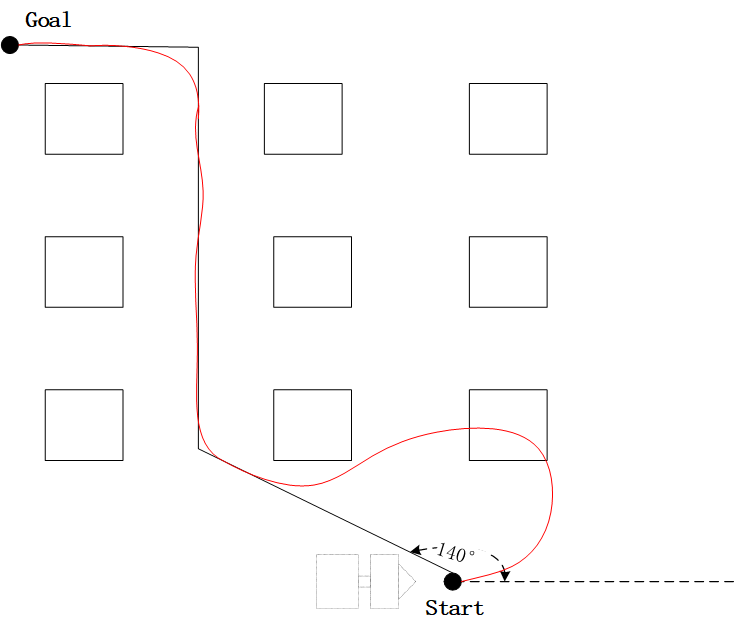
\includegraphics[width=0.8\textwidth]{路径规划算法特例.png}
			\caption{路径规划算法特例}
			\label{fig:路径规划算法特例}
		\end{figure}
		上图中时模拟一个路径规划算法的特殊例子,需要规划起点Start到终点Goal的路径。一般的算法可能规划出如图的路径,可以看到路径的起点切向和机器人的朝向相差140度。对于差速机器人跟踪这条路径的话,他会先原地转向然后继续跟踪其他点。对于全向机器人它直接可以顺着路径走,不必掉头。但是对于类车转向和铰接转向底盘,这两种底盘在转向时不仅有严格的非完整性,同时转向半径非常大。这会直接导致在开始的一段路径跟踪时会走出如图红色的路径,严重不贴合全局路径。这会带来出乎意料的后果,例如撞向障碍物或走出地图边缘。
		%然而,在具体的工作场景中,例如码头搬运任务,铰接车通常需要采用一种面向任务的路径规划方法。例如,车辆需要先到达A点进行货物装载,然后再前往B点进行卸货。/
		本章将基于优化理论和Minco样条,提出一种适用于铰接车辆的全局路径优化方法,可以在整段路径上保证严格的转弯半径约束并保证安全躲避碰撞。
		

	\section{铰接模型微分平坦性}
		\subsection{铰接车模型的平坦输出}
		在实际场景中情况是非常复杂的,全局的轨迹规划中我们不需要用精确的运动学模型。在这里我们忽略动态转向,只保留静态转向模型。假设 为系统输入,静态转向模型为:
		\begin{equation}
			\begin{aligned}
				\dot{\theta}=v\frac{tan( \gamma /2 )}{L}
			\end{aligned}
		\end{equation}
		对于一个非线性系统的动态方程具有如下一般的表达形式:
		\begin{equation}
			\begin{aligned}
				\dot{x}&=f( x,u ) ,x\in R^n,u\in R^m\\
			\end{aligned}
		\end{equation}
		其中$x$是状态变量,$f(x,u)$是系统的非线性函数。对于一个非线性系统,如果能找一组输出变量,使得所有的状态变量输出变量都可以用这组输出变量及其多阶导数所表示,则称这个系统为微分平坦系统。
		对于微分平坦的运动学模型,其平坦输出一般具有实际的物理意义往往会给问题带来很好的可表征性。对于铰接车的运动模型,我们选择$x,y$作为平坦输出,这在轨迹规划中可以带来很好的性质。
		下面我们给出装载机的微分平坦系统:
		\begin{equation}
			\begin{aligned}
				v&=\eta \sqrt{\dot{x}^2+\dot{y}^2},\\
				\theta &=arctan2( \eta \dot{y},\eta \dot{x} ) ,\\
				\gamma &=2arctan( \eta ( \dot{x}\ddot{y}-\dot{y}\ddot{x} ) L/( \dot{x}^2+\dot{y}^2 ) ^{\frac{3}{2}} ) ,\\
				k&=( \dot{x}\ddot{y}-\dot{y}\ddot{x} ) /( \dot{x}^2+\dot{y}^2 ) ^{\frac{3}{2}}.\\
			\end{aligned}
		\end{equation}
	其中$x,y$是系统的平坦输出变量,$(v,theta,gamma,k)$是我们选取的状态变量。k为轨迹的曲率,值得指出的是曲率其实也是铰接角的函数,但是这里只在路径层面说明。$n\in{1,-1}$是车辆运动的方向,分别代表前进和后退两种情况。
	\section{参数化轨迹表达形式}
	在自动驾驶中参数化曲线的方法有很多,例如五次多项式、贝塞尔曲线、B样条、螺旋线、Dubin曲线和RS曲线。MINCO曲线作为是一种基于五次多项式的曲线类型,它在处理微分平坦系统上有着天然的优势【文献】。我们这一小节将介绍minco曲线的原理,并且运用它处理我们的铰接模型运动规划问题。
		\subsection{MINCO曲线轨迹原理}
		铰接车在静态转向时表现出微分平坦性,这意味着其运动学微分约束可以通过一组平坦变量及其多阶导数来表示。在多项式规划中一个典型的BVP问题可以表示为:
		\begin{equation}
			\begin{aligned}
				min\int_0^T{v}(t) ^TWv(t) dt\\
				s.t. \ \ \ z^s(t) =v(t) ,\forall t\in \left[ 0,T \right] ,\\
				z^{\left[ s-1 \right]}( t_0 ) =\bar{z}_o,z^{\left[ s-1 \right]}( t_M ) =\bar{z}_f.
			\end{aligned}
		\end{equation}
		其中$z(t)$是参数曲线,$v(t)$是$z(t)$关于时间的$s$阶导数,$z_0$和$z_f$分别是起点和终点。对于以上最小控制输入问题,若系统是微分平坦的,且最小控制量是平坦变量的$s$阶次导数,则BVP问题的最优解是一个$2s-1$次多项式【文献】。特殊的,当$s=3$时这是一个minimumJerk(最小化加加速度代价)问题,他的最优解是一个五次多项式。 
		综上,轨迹曲线$z(t)$可以被表示为关于时间$t$多项式函数$\beta(t)$:
		\begin{equation}
			\begin{aligned}
				z=\beta (t) =\lambda ^T(t) c=c_0+c_1t+c_2t^2+c_3t^3+c_4t^4+c_5t^5\\
				=\left[ 1\,\,t\,\,\,\,t^2\,\,t^3\,\,t^4\,\,t^5 \right] \cdot \left[ c_0\,\,c_1\,\,c_2\,\,c_3\,\,c_4\,\,c_5 \right] ^T
			\end{aligned}
		\end{equation}
		其中$c$是多项式的系数向量。这个多项式由起点和终点的各阶状态量解出。假设轨迹的时间段是$T$,写成矩阵形式:
		\begin{equation}
			\begin{aligned}
				\left[ \begin{array}{c}
				x_s\\
				v_s\\
				a_s\\
				x_e\\
				v_e\\
				a_e\\
				\end{array} \right] =\left[ \begin{matrix}
				1&		0&		0&		0&		0&		0\\
				0&		1&		0&		0&		0&		0\\
				0&		0&		2&		0&		0&		0\\
				1&		T&		T^2&		T^3&		T^4&		T^4\\
				0&		1&		2T&		3T^2&		4T^3&		5T^4\\
				0&		0&		2&		6T&		12T^2&		20T^3\\
				\end{matrix} \right] \left[ \begin{array}{c}
				c_0\\
				c_1\\
				c_2\\
				c_3\\
				c_4\\
				\end{array} \right] ==>d=A_F(t) c
			\end{aligned}
		\end{equation}
		在上式中,$x_s,v_s,a_s$分别是轨迹起点的位置、速度和加速度,$x_e,v_e,a_e$对应为终点的状态。在实际的规划问题中为了保证轨迹的灵活性,轨迹规划被表述为多个BVP的总和,即BIVP问题:
		\begin{equation}
			\begin{aligned}
				\min_{z(t)}\int_{t_0}^{t_M}&v^T(t)\mathbf{W}v(t)dt\\
				\text{s.t}.z^{( s )}(t) &=v(t) \quad \forall t\in \left[ t_0,t_M \right]\\
				z^{\left[ s-1 \right]}( t_0 ) &=\bar{z}_o,z^{\left[ s-1 \right]}( t_M ) =\bar{z}_f\\
				z^{\left[ d_i-1 \right]}( t_i ) &=\bar{z}_i,1\leq i<M\\
				t_{i-1}&<t_i,1\leq i\leq M.\\
			\end{aligned}
		\end{equation}
		MINCO给出了这个BIVP问题的最优解形式,其最优性条件指出:对与最小化$s$阶导数的BIVP问题,他的最优解的单段轨迹一定是一个$2s-1$次多项式,且这个解具有$s+1$阶导数的连续性【文献】。这意味着我们在处理minimumJerk(s = 3)的轨迹时,这个轨迹具有snap阶(s = 4)阶的连续性,则BIVP问题的闭式解完全可以由起点状态、终点状态和中间位置所得到,如图..。
		\begin{figure}[!ht]
			\centering
			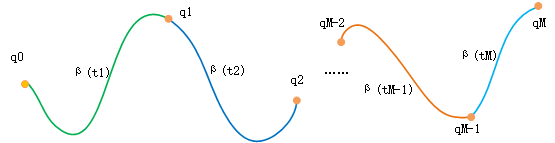
\includegraphics[width=0.8\textwidth]{minco.png}
			\caption{minco}
			\label{fig:minco}
		\end{figure}
	
		\subsection{轨迹参数化过程}
		假设我们共有$M+1$个航点$q_0~q_M$,其中起点$q_0=[x_s,y_s,v_{sx},v_{sy},a_{sx},a_{sy}]$和终点$q_M=x_e=[x_e,y_e,v_{ex},v_{ey},a_{ex},a_{ey}]$完全已知,需要求出M段多项式轨迹的表达式。  
		   
			A、起点和终点约束    
			  
			我们假设s=3,一个规划问题的起点和终点是已知的,起点和终点可以得到一共可以得到2s=6个约束方程,起点的约束方程为:
			\begin{equation}
				\begin{aligned}
				\left[ \begin{matrix}
					p_{0x}&		p_{0y}\\
					v_{0x}&		v_{0y}\\
					a_{0x}&		a_{0_y}\\
				\end{matrix} \right] =\left[ \begin{matrix}
					1&		0&		0&		0&		0&		0\\
					0&		1&		0&		0&		0&		0\\
					0&		0&		2&		0&		0&		0\\
				\end{matrix} \right] \left[ \begin{matrix}
					c_{0x}^{0}&		c_{0y}^{0}\\
					c_{1x}^{0}&		c_{1y}^{0}\\
					c_{2x}^{0}&		c_{2y}^{0}\\
					c_{3x}^{0}&		c_{3y}^{0}\\
					c_{4x}^{0}&		c_{4y}^{0}\\
					c_{5x}^{0}&		c_{5y}^{0}\\
				\end{matrix} \right] ==>b_0=F_0\cdot c_0
				\end{aligned}
			\end{equation}
			
			B、航点的连续性约束
			
			除了已知起点和终点之外,我们还必须保证BIVP问题中间航点的连续性。根据Minco的理论,minimumJerk问题(s=3)具有snap阶的连续性:
			\begin{equation}
				\begin{aligned}
					\left[ \begin{array}{c}
						\beta(t)\\
						\beta^{'}(t)\\
						\beta^{''}(t)\\
						\beta^{'''}(t)\\
						\beta^{''''}(t)\\
					\end{array} \right] &=\left[ \begin{array}{c}
						x(t)\\
						v(t)\\
						a(t)\\
						jerk(t)\\
						snap(t)\\
					\end{array} \right] =\left[ \begin{array}{c}
						\lambda_{t}^{T}\\
						\lambda_{t}^{( 1 ) T}\\
						\lambda_{t}^{( 2 ) T}\\
						\lambda_{t}^{( 3 ) T}\\
						\lambda_{t}^{( 4 ) T}\\
					\end{array} \right] \cdot \mathbf{c}=\left[ \begin{matrix}
						1&		t&		t^2&		t^3&		t^4&		t^5\\
						0&		1&		2t&		3t^2&		4t^3&		5t^4\\
						0&		0&		2&		6t&		12t^2&		20t^3\\
						0&		0&		0&		6&		24t&		60t^2\\
						0&		0&		0&		0&		24&		120t\\
					\end{matrix} \right] \cdot \mathbf{c}\\
					&\Longrightarrow G(t) \mathbf{c}=\mathbf{b}(t) 
				\end{aligned}
			\end{equation}
			因此第$i$段轨迹和第$i+1$段轨迹的连续性约束方程可以写为:
			\begin{equation}
				\begin{aligned}
					\left[ \begin{matrix}
						\beta ( T_i )&		0\\
						G( T_i )&		-G( 0 )\\
					\end{matrix} \right] \cdot \left[ \begin{array}{c}
						\mathbf{c}( i )\\
						\mathbf{c}( i+1 )\\
					\end{array} \right] =\left[ \begin{array}{c}
						\mathbf{b}( T_i )\\
						0\\
					\end{array} \right] \\
					\Longrightarrow \left[ E_i,F_i \right] \cdot \left[ \begin{array}{c}
						\mathbf{c}( i )\\
						\mathbf{c}( i+1 )\\
					\end{array} \right] =\left[ \begin{array}{c}
						\mathbf{b}( i )\\
						0\\
					\end{array} \right] 
				\end{aligned}
			\end{equation}
			综合起点、终点和航点的约束我们可以得到$2Ms$个约束方程,系数矩阵我们表示为M,由$M$和$b$可以唯一确定一组多项式系数$c$,即轨迹的参数形式。
			\begin{equation}
				\begin{aligned}
					M_{2Ms\cdot2Ms}\mathbf{c}=b\Longrightarrow ( \begin{matrix}
						\mathbf{F}_0&		0&		0&		\cdots&		0\\
						\mathbf{E}_1&		\mathbf{F}_1&		0&		\cdots&		0\\
						0&		\mathbf{E}_2&		\mathbf{F}_2&		\cdots&		0\\
						\vdots&		\vdots&		\vdots&		\ddots&		\vdots\\
						0&		0&		0&		\cdots&		\mathbf{F}_{M-1}\\
						0&		0&		0&		\cdots&		\mathbf{E}_M\\
					\end{matrix} ) \cdot \left[ \begin{array}{c}
						\mathbf{c}_1\\
						\mathbf{c}_2\\
						\mathbf{c}_3\\
						\vdots\\
						\mathbf{c}_{M-1}\\
						\mathbf{c}_M\\
					\end{array} \right] =\left[ \begin{array}{c}
						b_0\\
						b( 1 )\\
						0\\
						\vdots\\
						0\\
						b_M\\
					\end{array} \right] 
				\end{aligned}
			\end{equation}
			值得一提的是,在$M$矩阵中$T_i$是第$i$段多项式的总时间,它可以提前由一些其他的算法来给出,这样M就是完全已知的矩阵了。由于我们做的是路径规划,所以我们把$T_i$都归一化处理作为常数。
			
		\subsection{轨迹平滑与优化}
		常见的路径规划算法得到的路径是有拐角的,对于具有转向半径约束的车辆来说并不能完全的跟踪。因此在进行轨迹规划时必须考虑最大曲率的约束条件:
		\begin{equation}
			\begin{aligned}
				k_{max}=\frac{1}{R_{max}}=\frac{tan( \gamma _{max}/2 )}{L}
			\end{aligned}
		\end{equation}
	
	\section{基于安全走廊的安全约束分析}
	在上一节中我们已经对铰接车的轨迹进行了参数化,这样就自然的处理了微分方程带来的约束问题,保证了轨迹的平滑性。但是在路径规划中还有一个典型的问题需要处理,那就是障碍物躲避。无人车辆在非结构或半结构的场景中还需要面临安全性带来的种种挑战,包括避开其他工程机械车辆和环境中的种种障碍物。

	无人车的避障和地图的表示形式是分不开的,选择恰当的地图表示形式往往可以让避障算法发挥到很好的性能。常见的地图表示方法有占据栅格地图、点云地图、距离场、特征地图、拓扑地图、场图以及语义地图。规划算法中的避障部分一般根据地图的表示差异而有所不同。对于栅格地图而言,由于其均匀的栅格大小和快速的索引方式,使得它在几乎所有的避障算法中首当其冲,例如ROS(robot Operte sys。。)框架中就实现了基于栅格地图搜索的A*算法和Dijstra算法。点云地图是对空间中障碍物的直接表示,常见的激光slam算法建立的地图一般都是这种类型,基于此种地图的规划器一般需要结合KDTree(最近邻)搜索离当前位置最近的障碍物并避开。其次是特征地图,特征地图并不对整个地图空间进行离散,而是在地图上仅仅保留稀疏的特征。这些地图类型在不同的场景下有着不同的优势,针对某种类型的地图往往需要选择行之有效的规划器,减小规划的空间和时间复杂度。
	
	考虑到施工现场的结构不确定,往往地面上会有各种各样的杂物,为了充分利用栅格地图的快速索引能力并提高通用性,我们选择使用2维空间下的占据栅格地图作为规划的地图类型。
		\subsection{凸多边形约束的数学表达}
		对于凸包地图区间一般有两种表示方法,一种是把障碍物的轮廓用一个凸多边形近似模拟。另一种是则相反,将地图中安全的区域用凸多边形近似。在本次设计中,我们选择将地图安全区域用凸多边形来近似,这样铰接车的避障问题就转换为了铰接车是否在凸包内。
		% \begin{figure}[!ht]
		% 	\centering
		% 	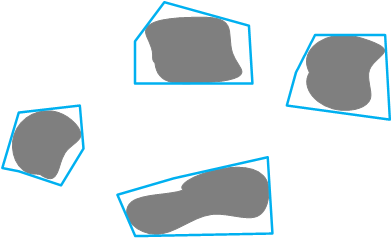
\includegraphics[width=0.8\textwidth]{凸包1.png}
		% 	\caption{凸包1}
		% 	\label{fig:凸包1}
		% \end{figure}
		% \begin{figure}[!ht]
		% 	\centering
		% 	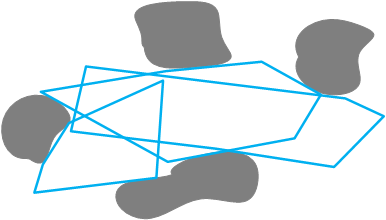
\includegraphics[width=0.8\textwidth]{凸包2.png}
		% 	\caption{凸包2}
		% 	\label{fig:凸包2}
		% \end{figure}
		凸多边形的表示方法有很多种类型,例如矩形和不规则凸多边形。在广义上,球体和椭球体也属于凸体。
		
		Gao等人使用固定方向的长方体安全走廊对轨迹进行优化,但是这种方法固定了安全走廊的拓展方向,在障碍物密集的环境中避障效果会大幅削弱\cite{Gao2018OnlineST}。Li等人提出的STC(Safe Travel Corridors)算法基于当前路径段的方向进行矩形迭代扩展,生成方式更加灵活\cite{BaiLi:2022}。Deits 等人提出了IRIS算法(Iterative Region Inflation by Semidefinite Programming),该方法通过不断膨胀椭球的长短半径,求得与障碍物的切平面,进而构造凸多面体\cite{Deits:2015}。每次迭代使用最大体积内接椭球作为起始点,然而此过程需要多次求解半正定规划,计算开销较大。Liu 等人提出了SFC算法(Safe Flight Corridors),该算法基于线段不断求解包含该线段且不与障碍物相交的最大椭球,并通过椭球与障碍物的切平面构建凸多面体,从而形成安全走廊\cite{SikangLiu:2017}。
		
		我们使用的空间表示体是不规则凸多边形,它的生成方法参考文献\cite{SikangLiu:2017}。它相较于矩形的可以把空间填充的更充实,更逼近于障碍物,从而带来更大的解空间。下图是矩形走廊和不规则凸包走廊的对比图。
		\begin{figure}[!ht]
			\centering
			\subcaptionbox{安全走廊比较矩形1\label{安全走廊比较矩形1}}[0.49\textwidth]{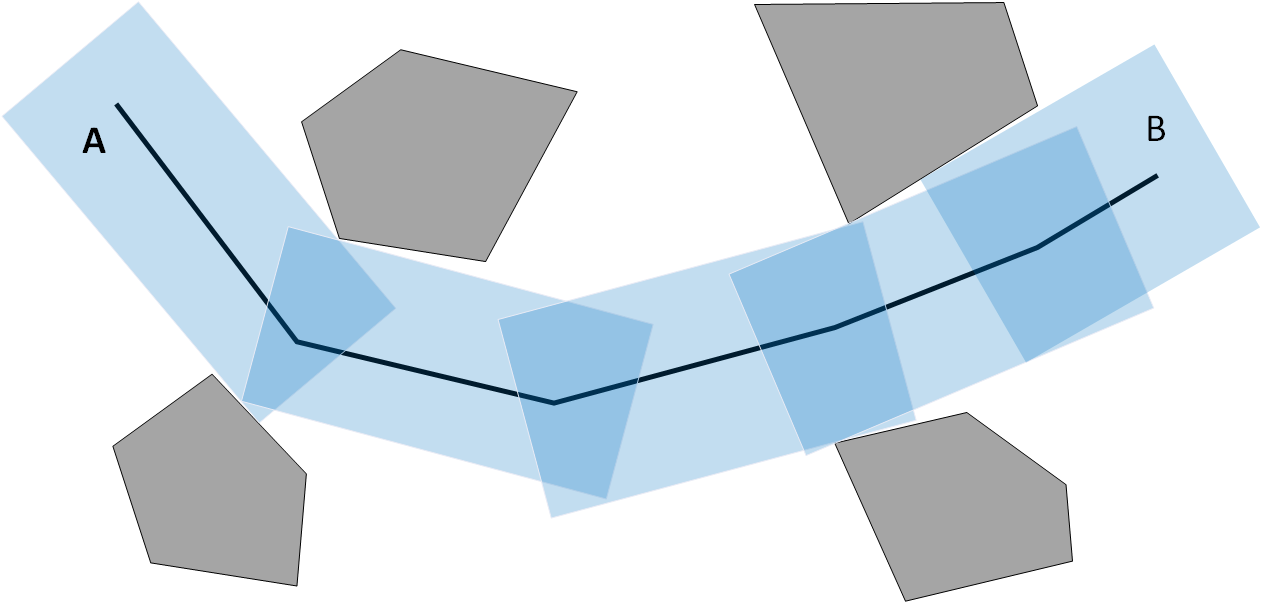
\includegraphics[width=0.4\textwidth]{安全走廊比较矩形1.png}}
			\subcaptionbox{安全走廊比较多边形2\label{安全走廊比较多边形2}}[0.49\textwidth]{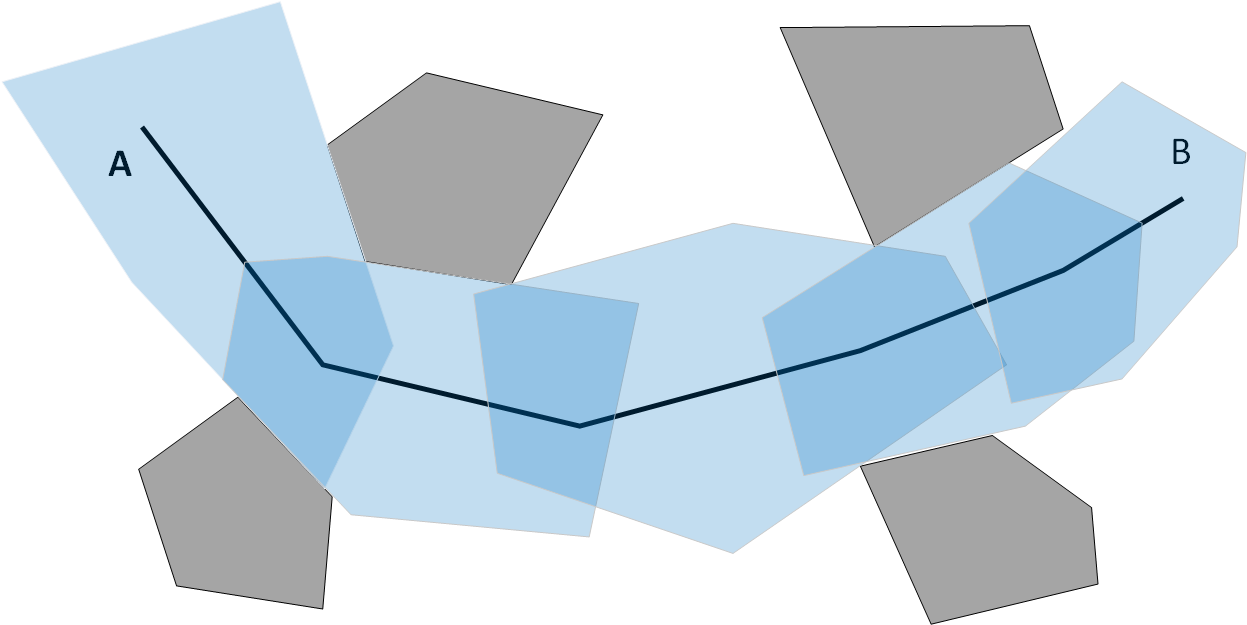
\includegraphics[width=0.4\textwidth]{安全走廊比较多边形2.png}}
			\caption{安全走廊的比较}
			\label{安全走廊比较}
		\end{figure}
		
		凸多边形的区域由一组半空间交集组成。对应2D场景凸包就是由一组直线围成的。如图\ref{fig:凸包矩阵}所示。
		\begin{figure}[!ht]
			\centering
			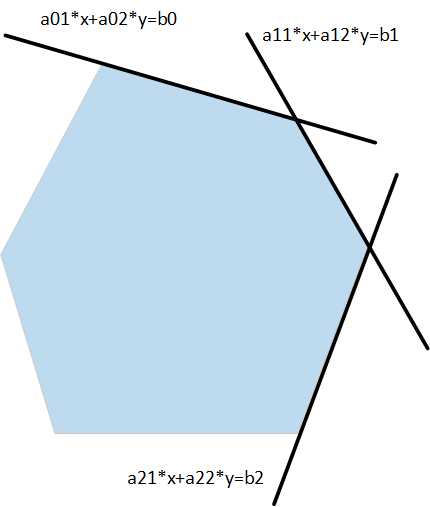
\includegraphics[width=0.4\textwidth]{凸包矩阵.png}
			\caption{凸包的数学表达关系}
			\label{fig:凸包矩阵}
		\end{figure}
		因此,在封闭区域内的点必然满足以下不等式约束:
		\begin{equation}
			\begin{aligned}
				H_z&=\{p\mid Ap<b\},\\
				A&=\left[ a_0,...,a_z,...a_{n_z-1} \right]^T_{(n_z-1)\times 2},b=\left[ b_0,...,b_z,...,b_{n_z-1} \right]^T_{(n_z-1)\times 1}.
			\end{aligned}
		\end{equation}
		其中$a_i$是第$i$个半空间的法向量,$a_i$和$b_i$唯一去确定一个超平面约束。对于任意在多边形内的点应当满足【等式】带来的不等式约束。多边形的生成方法参考文献【】。
	
	\section{单阶段无约束轨迹规划}
	在3.2中我们介绍了MINCO曲线的参数化形式。由于我们在这一章介绍的全局的路劲规划,所以我们只关心路径层面信息包括曲率和避障。路径的最大曲率,这由装载机的最大转向角推导得到。避障我们在3.3节我们已近介绍。
		\subsection{优化问题的建立}
		针对于这个问题我们使用优化的方法解决,我们把曲率和安全约束离散化的施加在问题中,当离散化的点足够多时轨迹就是足够安全的。我们可以得到以下优化问题的表达形式:
		\begin{equation}
			\begin{aligned}
				&\min J( c )=0 \\
				s.t.\,\,&-k_{max}\le k_{ij}\le k_{max} \\
				&A_ip_{ij}<b_i,\ \ i\in \left[ 1,N \right] ,j\in \left[ 1,m_i \right] 
			\end{aligned}
		\end{equation}
		其中$c$轨迹多项式是系数矩阵,$K_{max}$是最大曲率,$N$是轨迹的段数,$m_i$是第$i$段轨迹的离散点数,$p_{ij}$是第$i$点轨迹的第$j$个点。
		\subsection{曲率约束和避障约束的消除}
		忽略动态转向带来的曲率影响,铰接式车辆的最大曲率由静态转向模型确定。本次设计中我们的最大转向角度为30度,轴距$L$为1.3,即最大转向半径为4.85m,最大曲率为0.2。
		曲率在二维平面上的公式为:
		\begin{equation}
			\begin{aligned}
				k=( \dot{x}\ddot{y}-\dot{y}\ddot{x} ) /( \dot{x}^2+\dot{y}^2 ) ^{\frac{3}{2}}
			\end{aligned}
		\end{equation}
		令$p =[x,y]^T$,则:
		\begin{equation}
			\begin{aligned}
				k\,\,=\,\,\frac{\ddot{p}^TB\dot{p}}{\lVert p \rVert _{2}^{3}},B\,\,=\,\,\left[ \begin{matrix}
					0&		-1\\
					1&		0\\
				\end{matrix} \right] .
			\end{aligned}
		\end{equation}
		\begin{equation}
			\begin{aligned}
				\frac{\partial k}{\partial \dot{p}}\,\,=\,\,\frac{B^T\ddot{p}}{||\dot{p}||_{2}^{3}}-3\frac{\ddot{p}^TB\dot{p}}{||\dot{p}||_{2}^{5}}\dot{p},\frac{\partial k}{\partial \ddot{p}}=\frac{B\dot{p}}{||\dot{p}||_{2}^{3}}
			\end{aligned}
		\end{equation}
		针对于曲率和安全这两个不等式约束,我们引入一个松弛函数将它们最为软约束加入到代价中,松弛函数为:
		\begin{equation}
			\begin{aligned}
				S( x ) =\left\{ \begin{matrix}
					0&		x\le 0,\\
					-\frac{1}{2a^3}x^4+\frac{1}{a^2}x^3&		0<x\le a\\
					x-\frac{a}{2}&		a<x.\\
				\end{matrix} \right.  \\
					S^{'}(x) = \left\{\begin{matrix}
					0& x\le0, \\
					-\frac{2}{a^3}x^3+\frac{3}{a^2}x^2& 0 < x \le a \\
					1& a < x.
				\end{matrix}\right.
			\end{aligned}
		\end{equation}
		其中a是一个参数,我们一般选取为优化问题迭代的停止条件值。下面是这个分段函数的图像信息,【函数、导数图像】。
		\begin{figure}[!ht]
			\centering
			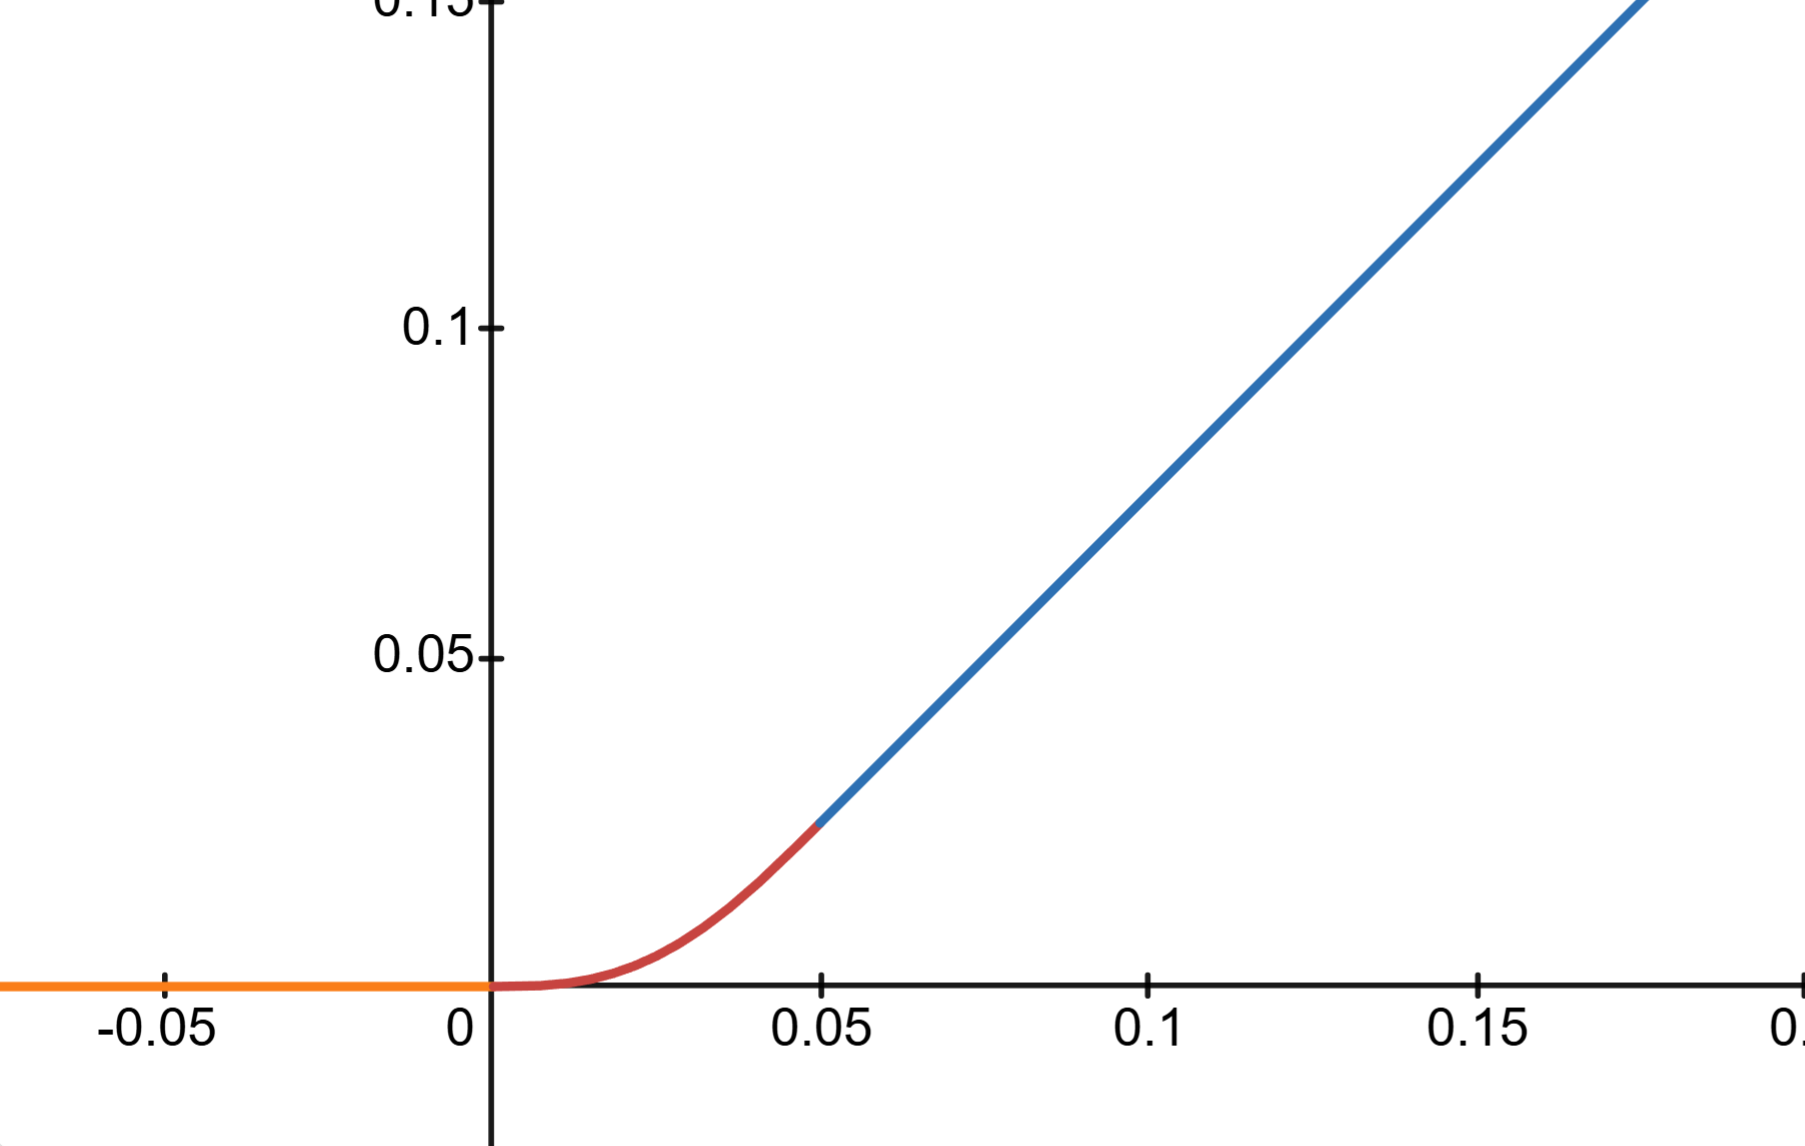
\includegraphics[width=0.8\textwidth]{松弛函数.png}
			\caption{松弛函数}
			\label{fig:松弛函数}
		\end{figure}
		\begin{figure}[!ht]
			\centering
			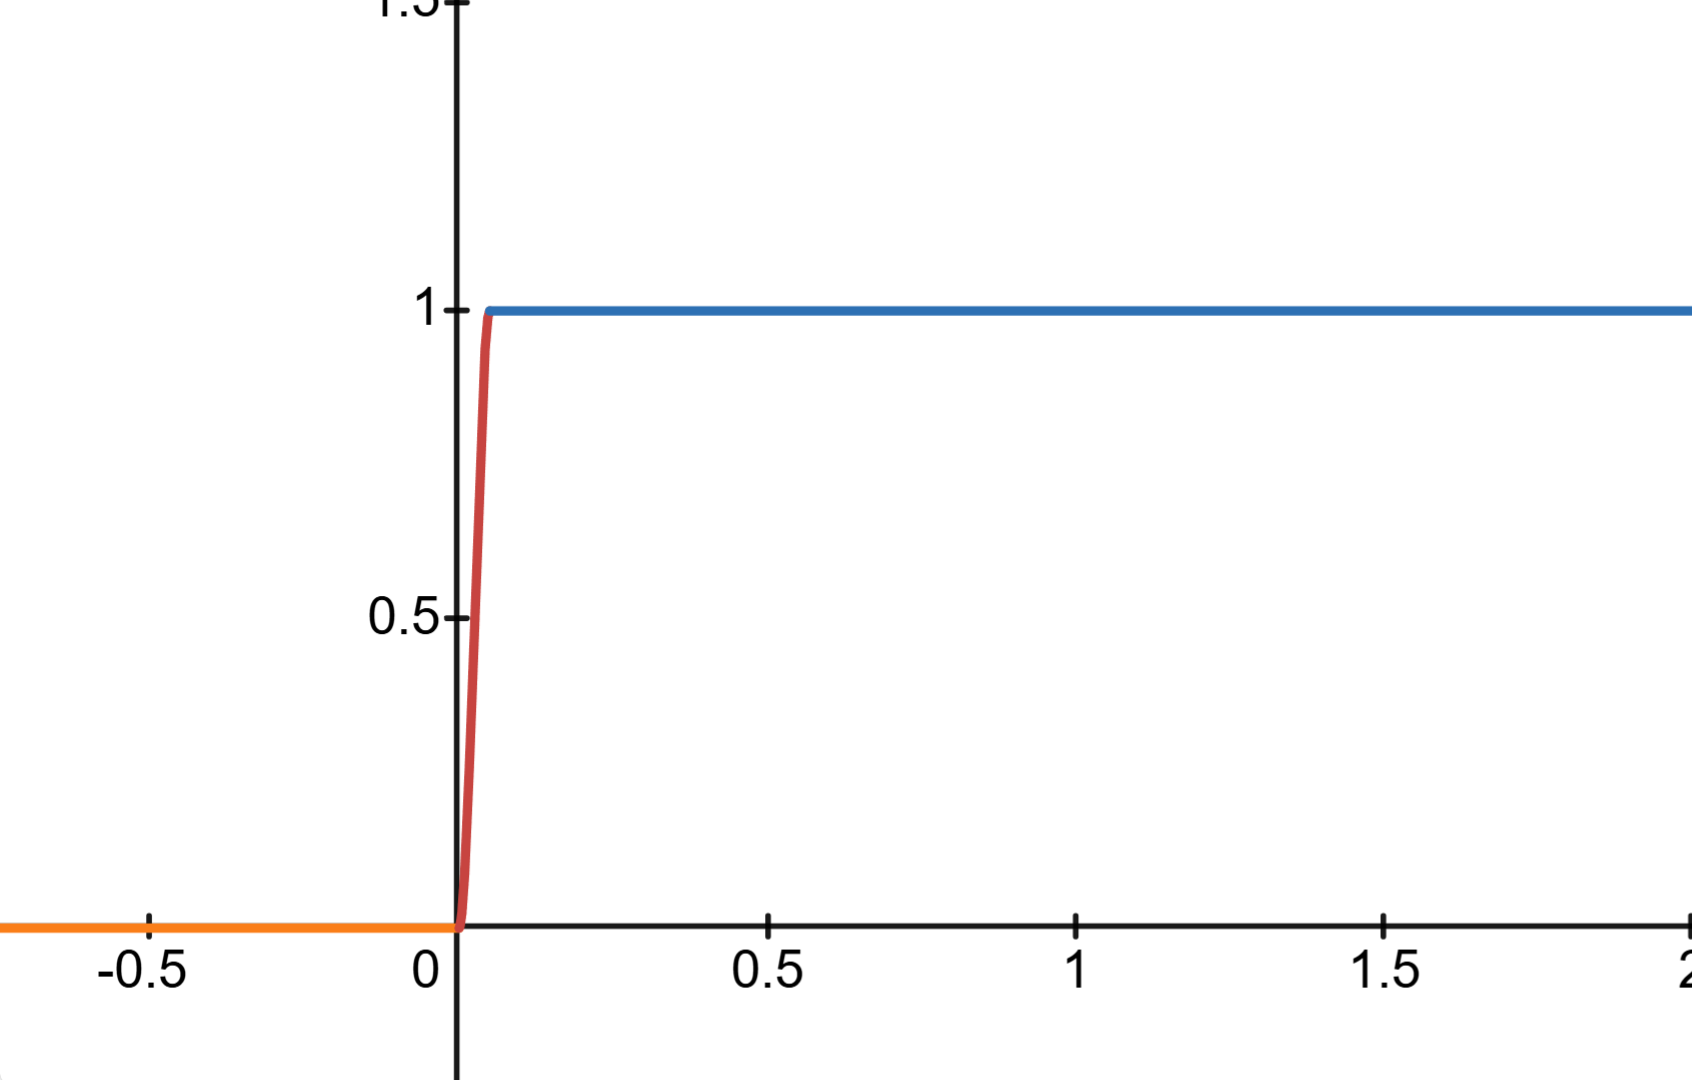
\includegraphics[width=0.8\textwidth]{松弛导数.png}
			\caption{松弛导数}
			\label{fig:松弛导数}
		\end{figure}
		我们设置的a=0.05。可以看出这个函数在x的负半轴的值为0,也就意味着不等式约束的代价为0。在0<x<=a时代价以一个四次函数上升,越靠近原点代价越小。当x>a时代价值以斜率为1直线上升。另外这个分段函数还有非常好的一个特性,在定义域上市C2微分同胚的。这就意味着它的梯度和Hessian矩阵是完全连续的,在优化时我们不必考虑额外的光滑函数。
		综上,问题被化简成了一个无约束的优化问题:
		\begin{equation}
			\begin{aligned}
				\min\text{\ }J( q ) \ =\ \sum_{i=1}^N{\sum_{j=1}^{m_i}{S( -k_m-k_{ij} ) +S( -k_m+k_{ij} ) +S( A_ip_{ij}-b_i )}}
			\end{aligned}
		\end{equation}
		利用矩阵求导的链式法则我们可以求得各个部分的梯度信息,需要指出的是我们矩阵求导遵循分母布局。
		\begin{equation}
			\begin{aligned}
				\frac{\partial S( -k_m-k_{ij} )}{\partial c_i}&=-( \frac{\partial \dot{p}_{ij}}{\partial c_i}\frac{\partial k_{ij}}{\partial \dot{p}_{ij}}+\frac{\partial \ddot{p}_{ij}}{\partial c_i}\frac{\partial k_{ij}}{\partial \ddot{p}_{ij}} ) S^{'} ( -k_m-k_{ij} ) ,\\
				\frac{\partial S( -k_m+k_{ij} )}{\partial c_i}&=( \frac{\partial \dot{p}_{ij}}{\partial c_i}\frac{\partial k_{ij}}{\partial \dot{p}_{ij}}+\frac{\partial \ddot{p}_{ij}}{\partial c_i}\frac{\partial k_{ij}}{\partial \ddot{p}_{ij}} ) S^{'} ( -k_m+k_{ij} ) \\
				\frac{\partial S( A_ip_{ij}-b_i )}{\partial c_i}&=\frac{\partial p_{ij}}{\partial c_i}A_{i}^{T}S^{'}( A_ip_{ij}-b_i ) 
			\end{aligned}
		\end{equation}
		我们利用上式求出了$J$关于$c$的梯度$\frac{\partial J}{\partial q}=\frac{\partial c}{\partial q}\frac{\partial J}{\partial c}$,于是由$b = Mc$,可以推导出:$\frac{\partial b}{\partial q}M^{-T}=\frac{\partial c}{\partial q}$ ,因此$J$关于$q$的梯度为:
		\begin{equation}
			\frac{\partial J}{\partial q}=\frac{\partial c}{\partial q}\frac{\partial J}{\partial c}
		\end{equation}
		
		
		\subsection{优化结果的分析}
		通过上一小节我们推出了路径优化问题的代价函数和梯度信息,这是很关键的。求解无约束优化问题的优化方法有很多,例如最速下降法、牛顿法、共轭梯度法等。对于一般的优化算法而言总体上可以分为两类,一类是基于一阶信息的梯度法,另一类是基于二阶信息的牛顿法。牛顿法除了需要提供代价函数的梯度信息以外,还需要提供代价函数的Hessian矩阵。对于复杂优化问题而言解析计算Hessian是极为复杂的。综合众多因素我们选择使用lbfgs优化算法最为本优化问题的优化求解算法。
		LBFGS算法作为一种高效的拟牛顿优化方法,在优化过程中会不断地迭代逼近出一个Hessian矩阵,省去了手动推导的难度。在大规模无约束优化问题中展现出显著的优势。其核心优势在于内存效率和计算效率,仅存储最近的迭代信息,有效处理高维问题,同时快速收敛于最优解。LBFGS算法的适用性广泛,覆盖机器学习、统计学和工程优化等多个领域,尤其在大规模数据处理中表现出色。
		由于使用优化的方法生成轨迹,所以我们需要一个快速生成航点的路径规划算法,为我们的优化算法提供软起动初值。我们不关心这个算法是否路径最优,但是它需要以较低的时间复杂度运行,因为我们的优化过程可以带来足够的最优性。下面给出我们算法的伪代码:
		 \begin{algorithm}[H]  
		 	\caption{Global Planning}  
		 	\label{Planning}  
		 	\begin{algorithmic}[1]  
		 		\REQUIRE  
		 		$\mathbf{p_{start}},\mathbf{p_{end}},\mathbf{map}$
		 		\ENSURE  
		 		$\mathbf{path}$
		 		\STATE $\hat{path} \leftarrow RRTConnect(\mathbf{p_{start}},\mathbf{p_{end}},\mathbf{map})$
		 		\STATE $cors \leftarrow getCorridor(\mathbf{map},\hat{path})$
		 		\STATE $cons \leftarrow getConstraint(\kappa_{min,max},cors)$
		 		\STATE $costFcn \leftarrow getCost(cons)$
		 		\STATE $grad \leftarrow getGrad(cons)$ \\
		 		\RETURN $\mathbf{path} \leftarrow \mathbf{lbfgs}(costFcn,grad)$
		 	\end{algorithmic}  
		 \end{algorithm}
		 在这里我们推荐使用RRTConnect或者JPS算法,这两者都具有快速生成路径的能力。以下介绍的所有例子都是用RRTConnect生成路径。区别于传统的RRT算法,RRTConnect同时从起点和终点搜索路径,可以显著提高搜索的效率,减少搜索的次数。
		 \begin{figure}[!ht]
		 	\centering
		 	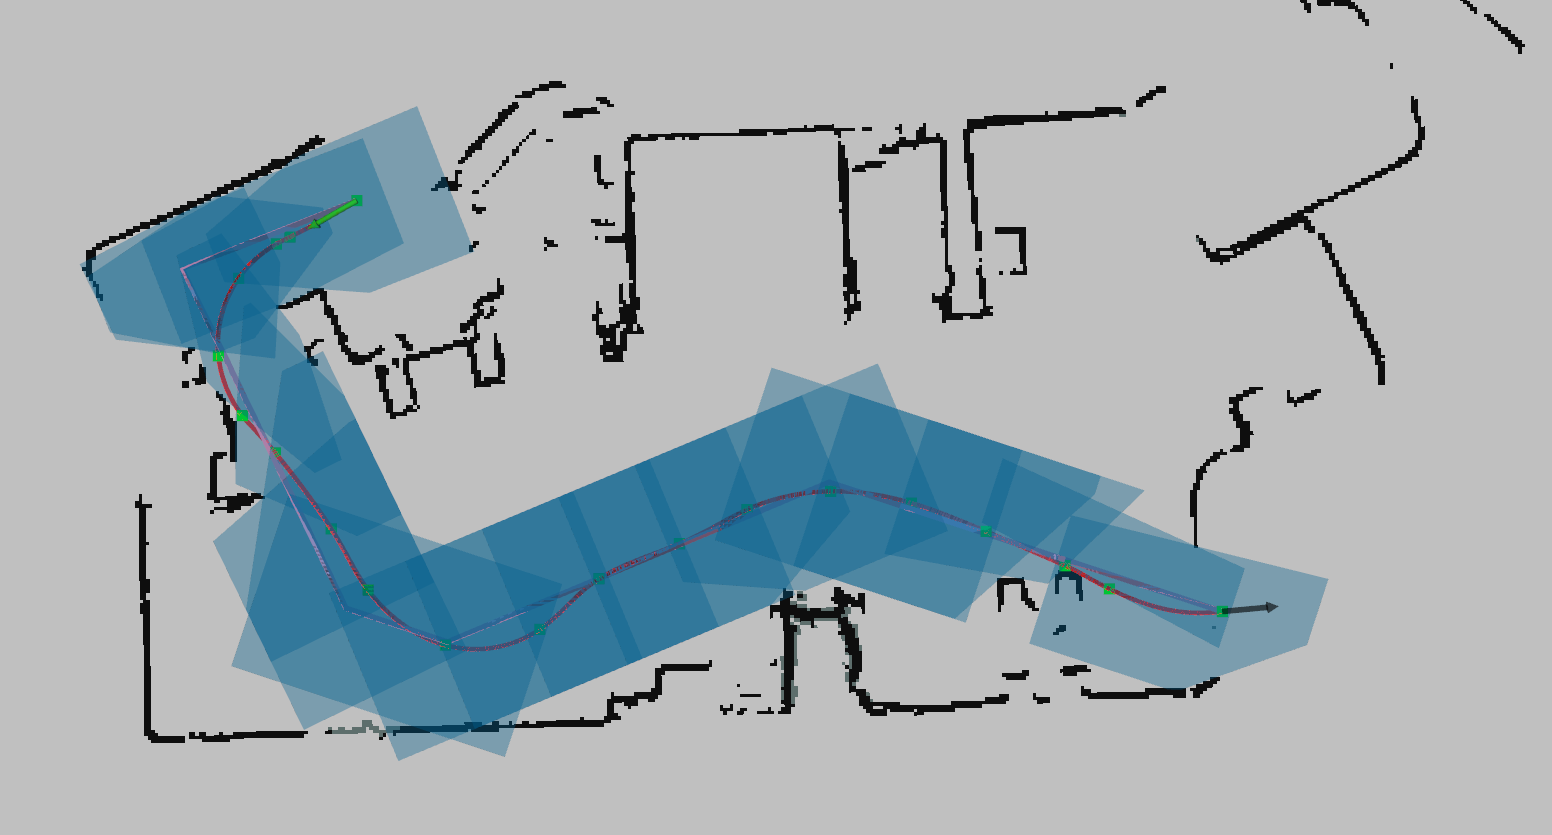
\includegraphics[width=0.8\textwidth]{单轨迹2.png}
		 	\caption{单轨迹2}
		 	\label{fig:单轨迹2}
		 \end{figure}
		 图。。。。是的算法运行的仿真,其中浅紫色那条路径是RRTConnect搜索出的初始路径,他在全局范围内是无碰撞的。沿着初始路径我们生成了如图蓝色的安全走廊,用来表示路径周围的FreeSpace。绿色的点是优化后的航点。红色的是我们优化之后的轨迹,可以看出它严格符合事先给出的曲率约束,并且在完全处于安全走廊内。
		
	\section{多阶段全局轨迹规划案例}
	在上一节中我们描述了一个完整的全局轨迹规划算法,可以完成一个点对点的路径规划问题。对于一些更加复杂的场景,例如码头搬运、舱体清卸、矿山运料等多种复杂的工况下,铰接车需要依次去往各个区域规定完成卸货。这样的场景往往需要面向任务设计一个框架。因为这些场景需要更灵活的运动模式,例如倒车。这一节我们将针对码头搬运场景设计一个周期性的规划流程。
	\begin{figure}[!ht]
		\centering
		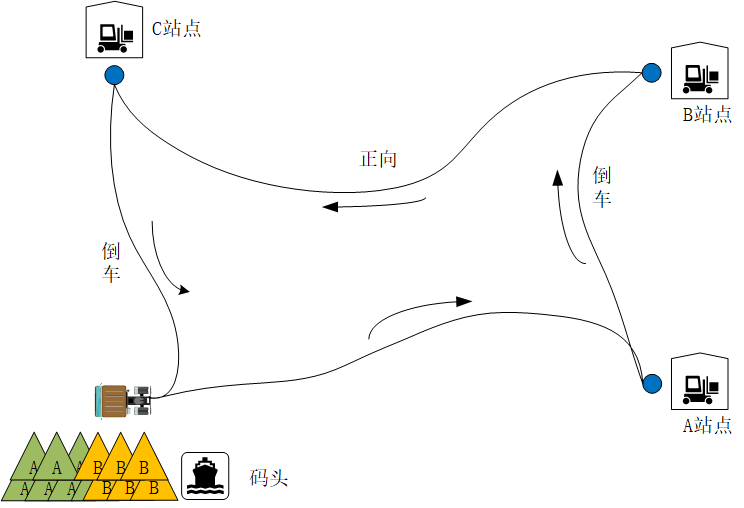
\includegraphics[width=0.8\textwidth]{全局规划.png}
		\caption{全局规划}
		\label{fig:全局规划}
	\end{figure}
		\subsection{多阶段规划的问题描述}
		考虑【如图】的搬运问题,我们需要铰接车从起点码头装货完成去往A点进行卸货,然后去往B点,再去C点,最后回到码头重新装货。这个搬运周期一共需要四次规划,且搬运过程中由于环境等因素规划过程需要倒车。
		\subsection{航点过渡策略}
		在整个规划周期中铰接车一共需要经过四个航点,分别为码头、A站点、B站点和C站点。在整个过程中受到路径受到两个方面的限制。第一,每一段轨迹的起点的切线方向必须和铰接车保持一致,这可以由曲率约束所保证。第二,如果在航点处需要求车辆发生换向,则换向后的轨迹的航向和换向前应该相反。 
		
		A、轨迹起点和初始位姿一致性保证
		由于我们使用minco对x和y方向分开规划,所以铰接车的初始位姿要同时作用在x和y两个方向上。记初始的姿态为$\theta_s$ ,由运动学模型我们可以求得:
		\begin{equation}
			v_{sx}=v_scos\theta _s\\
			v_{sy}=v_ssin\theta _s
		\end{equation}
		对于初始速度$v_s$不为零的情况,$v_{sx},v_{sy}$都不等于零,我们带入优化问题就可以直接保证车辆初始朝向和轨迹的起点切向在一条直线上。但是当$v_{s}=0$时,推出$v_{sx}=0,v_{sy}=0$。此时用平坦模型计算$\theta_s$:
		\begin{equation}
			\theta_s=\text{atan}2\left( v_{sy},v_{sx} \right) =\text{atan}2\left( 0,0 \right) 
		\end{equation}
		我们发现其实当$v_{s}=0$时曲线的切线方向是没有定义的,这是一个奇异点。为了处理这种奇异情况,我们给当$v_{s}$加上一个微小正量保证它的有效性:
		\begin{equation}
			\begin{aligned}
			v_{sx}&=\left( v_s+\epsilon \right) cos\theta_s\\
			v_{sy}&=\left( v_s+\epsilon \right) sin\theta_s,0<\epsilon <1e-5.
			\end{aligned}
		\end{equation}
		这样就可以保证车辆的起点朝向施加在轨迹上,同样由于$\epsilon$是一个极小量,它几乎不会影响轨迹起点的初始速度。对于终点的处理方法和起点一样。
		
		B、航点的换向处理
		
		在中间航点处的是否换向包含两种情况,一种是航点前的车辆运动方向和航点后运动方向相同,则不需要换向。另一种是航点前的车辆运动方向和航点后运动方向相反,则需要换向,此航点也被称为换向点。
		\begin{figure}[!ht]
			\centering
			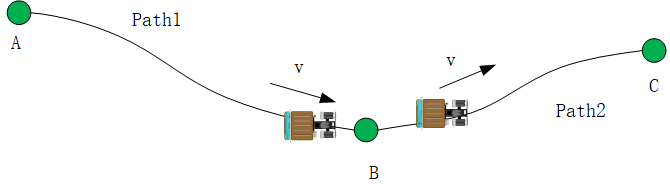
\includegraphics[width=0.8\textwidth]{换向1.png}
			\caption{换向1}
			\label{fig:换向1}
		\end{figure}
		\begin{figure}[!ht]
			\centering
			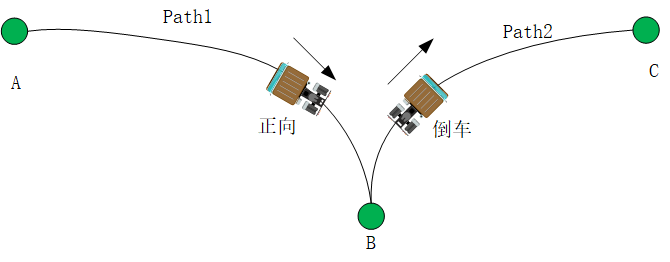
\includegraphics[width=0.8\textwidth]{换向2.png}
			\caption{换向2}
			\label{fig:换向2}
		\end{figure}
		图【】是表示的是车正向行驶穿越航点的情况,经过航点时不用倒车。我们在规划AB段路径时B点作为终点,在规划BC段路径时B点作为起点车辆的运动方向和车辆的朝向相同。图【】是表示的是车正向行驶到达航点,再反向倒车。与图【】不同的是,在规划BC段路径时B点作为起点车辆的运动方向和车辆的朝向相反,而AB段相同,因此规划BC段时B点作为起点需要反向。
		\subsection{规划结果展示}
		下面是我们算法在码头地图中的多阶段规划例子:
		\begin{figure}[!ht]
			\centering
			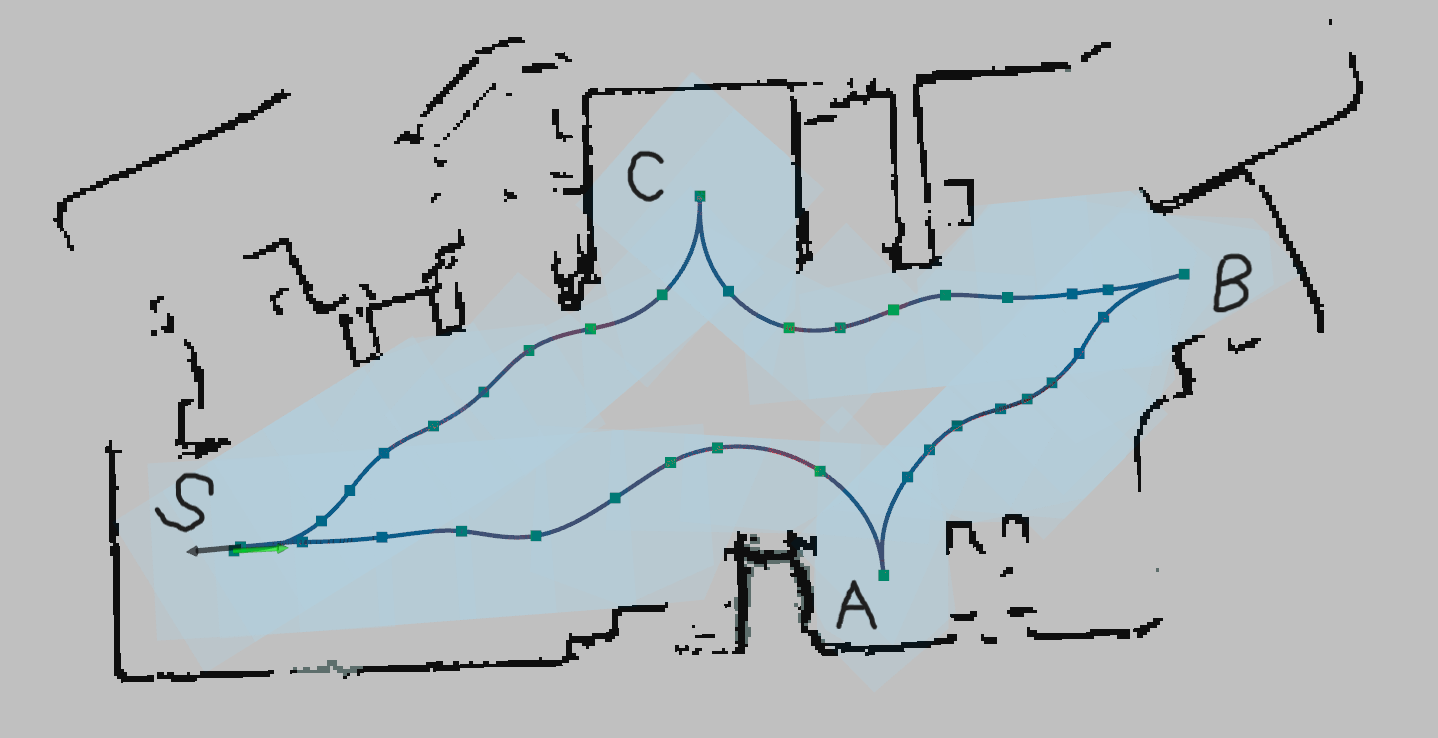
\includegraphics[width=0.8\textwidth]{多阶段轨迹s.png}
			\caption{多阶段轨迹s}
			\label{fig:多阶段轨迹s}
		\end{figure}
	\section{本章总结}
	在这节中我们介绍了铰接车的微分平坦模型,并使用minco参数化了我们轨迹的形式。然后我们分析了轨迹的安全约束和曲率约束。最后我们建立了一个点对点的规划问题,并给出了一个码头搬运的小案例。
	
	
	\chapter{基于安全走廊的无人铰接车局部规划方法}
	在这一章中我们主要介绍一种基于安全走廊的时空联合轨迹规划方法,这种方法采用最优控制(Optimal Control)的框架对问题建模。第一节中我们将对铰接车外观做一个通用性的建模,可以有效加强碰撞检测的速度。第二节中介绍针对于铰接车改进的Hybrid A*算法,它将用于我们轨迹规划算法的热启动。第三节介绍规划问题中涉及到的所有约束并进行处理。第四节我们对优化问题进行求解。
	\section{铰接车的一般性结构建模}
	为了保持优化问题的凸性,将车辆底盘形状建模为两个矩形的连接,从而将装载机的避障问题转化为多边形几何碰撞问题。车辆形状分为前轴和后轴两部分,共由九个顶点A,B,C,…,H和O1。这些顶点在车辆车身坐标系中的表示如下:
	\begin{figure}[!ht]
		\centering
		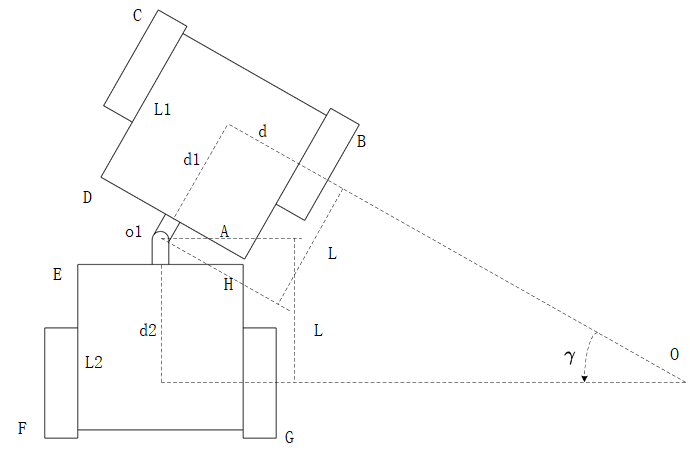
\includegraphics[width=0.8\textwidth]{ppi.png}
		\caption{ppi}
		\label{fig:ppi}
	\end{figure}
	与动学模型相一致,我们选取前后中点作为参考点$(x_f,y_f)$,沿着车体方向作为x轴正方向。则A,B,C,…,H和O1的相对坐标可以表示为:
	\begin{equation}
		\begin{aligned}
			l_{A}^{T}&=( -d_1,-width/2 ) ,l_{B}^{T}=( L_1-L,-width/2 ) ,\\
			l_{C}^{T}&=( L_1-L,width/2 ) ,l_{D}^{T}=( -d_1,width/2 ) ,\\
			l_{E}^{T}&=( d_2-L,width/2 ) ,l_{F}^{T}=( -L_2,width/2 ) ,\\
			l_{G}^{T}&=( -L_2,-width/2 ) ,l_{H}^{T}=( d_2-L,-width/2 ) ,\\
			l_{O_1}^{T}&=( -L,0 ) .\\
		\end{aligned}
	\end{equation}
	其中,lA,lB,lC,lD,lo1表示相对于底盘前桥坐标系下的坐标。lE,lF,lG,lH是相对于铰接点坐标系下的坐标。在世界坐标系中,坐标可以表示为旋转矩阵$R_\theta$和平移向量$\sigma$的组合。因此,根据(6),前轴的顶点集表示如下
	\begin{equation}
	\begin{aligned}
		\varepsilon_f = \left\{ p_f \in \mathbb{R}^2 \mid p_f=R_\theta l_f+\sigma,  f = A,B,C,D \right\},
	\end{aligned} 
	\end{equation}
	
	在这里$\sigma$表示前轴参考点坐标,表示为$\sigma=(x_f,y_f)$。在从世界坐标系到铰接点坐标系的变换中,还涉及到车身坐标系,需要应用旋转矩阵$R_\theta$和$R_\gamma$。平移向量由世界坐标系中的铰接点给出,记为$\sigma_1$。在(5)中,模型各点的坐标变换可表示为:
	\begin{equation}
		\begin{aligned}
			&\left\{\begin{matrix}
				p_r=R_\gamma R_\theta l_b+\sigma_1\\
				\sigma_1=R_\theta l_{O_1}+\sigma
			\end{matrix}\right.   \Longrightarrow \varepsilon_r ,\\
			&\varepsilon_r = \left\{ p_r \in \mathbb{R}^2 \mid p_r=R_\gamma R_\theta l_r+R_\theta l_{O_1}+\sigma,  \right\} ,\\
			&r = E,F,G,H.
		\end{aligned}
	\end{equation}
	
	\section{铰接车Hybrid A*算法的创新改进}
	在大规模优化问题中,影响求解质量的主要因素往往不是问题或约束的非线性特性,而是问题是否具备凸性。遗憾的是,大多数非线性规划问题都不具备凸性,只有少数问题能够通过对偶方法、变换等手段转化为凸优化问题。直接求解这类问题时,常常会陷入局部最优解,难以保证找到全局最优解。然而,对于这些非凸问题,我们依然可以采用其他思路,找到最优解或一个较为理想的解。关键在于,尽管问题本身无法严格保证非凸性,我们仍然可以使用一些全局最优算法,通过寻找一个接近最优的初值来确保其位于全局最优解所在的凸空间内。接下来,优化算法可以沿着这个初值在局部凸空间内展开迭代,最终找到最优解。
	例如,在百度Apollo的轨迹规划中,轨迹优化基元采用了多项式形式,通过优化控制点来生成满足要求的轨迹。在此过程中,控制点的初值是通过动态规划搜索得到的。动态规划的作用在于,通过对状态空间的逐步分解,找到一个合理的凸空间,使得优化算法能够高效地进行局部最优解的搜索。
	Hybrid A star算法首次应用于2007年DAPPA城市挑战赛,并由Dolgov等人提出。与传统的A star算法不同,Hybrid A star算法在三维空间中进行搜索,且在搜索过程中,邻居节点的拓展是通过动力学方程的前向推演来实现的。然而,传统的Hybrid A star算法是基于$x-y-\theta$三维空间进行搜索的,这使得它并不适用于铰接车模型。铰接车由于其具有较为复杂的非线性运动特性,因此直接应用传统的Hybrid A*算法会面临难以满足约束条件和路径质量不高的问题。
	为了使Hybrid A star算法能够适应铰接车的路径规划问题,本节将提出一种创新性的改进方法。具体来说,我们将修改Hybrid A算法中的邻居节点拓展策略,结合铰接车的运动学特性,改进算法的搜索策略,以便更好地在铰接车的状态空间中找到一个次优的初解。该初解将在后续的优化过程中作为起点,进一步引导算法沿着合适的方向优化,最终得到一个更加符合实际需求的路径。通过这种方式,我们能够克服传统Hybrid A*算法的局限性,为铰接车路径规划提供更为高效和精准的解决方案。
		\subsection{节点拓展策略改进}
		铰接车的位形(configuration)传统汽车有显著差异,其位形不仅依赖于车辆的位置和方向$(x,y,\theta)$,还受到铰接角$(gamma)$的影响。假设铰接车当前的状态为$x_0(x,y,\theta,\gamma)$,一般的hybrid算法将控制区间$[-v_{max},v_{max}]$和$[-\omega_{max},\omega_{max}]$进行离散化。并从当前状态$x_0$开始以输入采样值$[v,\omega]$在$\Delta_t$时间内进行运动学推演得到下一个状态,运动学推演见公式a,推演过程如图a。
		\begin{figure}[!ht]
			\centering
			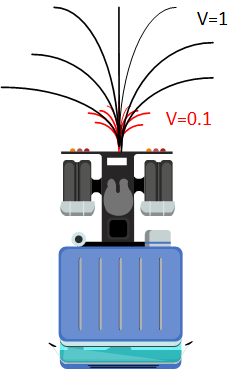
\includegraphics[width=0.5\textwidth]{hybrid采样.png}
			\caption{hybrid采样}
			\label{fig:hybrid采样}
		\end{figure}
		图a只简单列出了速度为0.1和1的情况。可以看出这种采样方式在$|v|$很小时,不管$\omega$为多少,所积分出来的轨迹都会聚在一起。如图a中的红色轨迹有短又聚合,并没有充分的去探索周围空间。这是很浪费计算资源且没有必要的。第二,由于系统的输入是二维$(v,omega)$,所以算法的时间复杂度是$O(N^2)$。下面我将针对节点采样进行改进,可以有效解决采样出来的轨迹聚合的问题,并以$O(N)$时间复杂度完成探索,某种意义上这也是一种轨迹的剪枝策略。 
		首先我们为了降低计算的复杂度,我们只使用铰接车的静态转向模型,系统的输入为$(v,\gamma_u)$。我们不再以固定的时间$\Delta_t$进行采样,我们以固定的行驶路程$\Delta_s$采样,于是系统的输入就只有$\gamma_u$。这样做的本质是只在路径几何层面考虑规划问题。运动学推演方程如下:
		\begin{equation}
			\begin{aligned}
				\left[ \begin{array}{c}
					x_{k+1}\\
					y_{k+1}\\
					\theta _{k+1}\\
					\gamma _{k+1}\\
				\end{array} \right] =\left[ \begin{array}{c}
					x_k+\Delta s\cdot cos\theta _k\\
					y_k+\Delta s\cdot sin\theta _k\\
					\theta _k+\frac{\Delta s}{L}\cdot tan (\gamma _{uk}/2 )\\
					\gamma _{uk}\\
				\end{array} \right] 
			\end{aligned}
		\end{equation}
		其中$\Delta s$是采样的路径步长,$(x,y,theta,gamma)$是铰接车的位形空间状态变量。$\Delta s$等于2m的推演过程如图b。
		\begin{figure}[!ht]
			\centering
			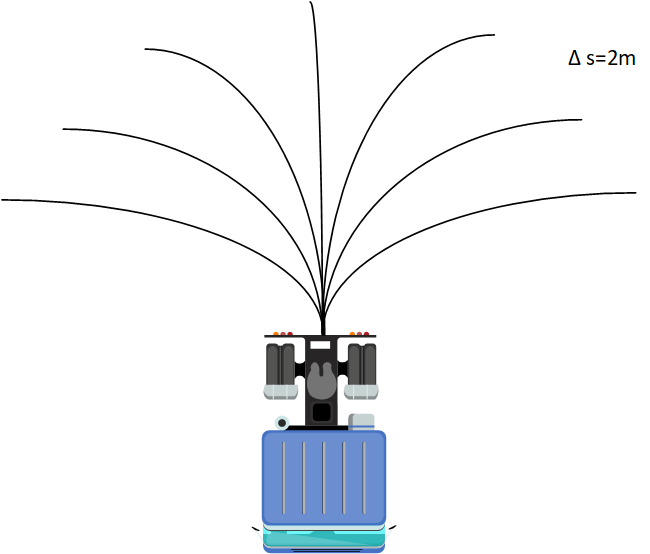
\includegraphics[width=0.8\textwidth]{hybrid采样改进剪枝.png}
			\caption{hybrid采样改进剪枝}
			\label{fig:hybrid采样改进剪枝}
		\end{figure}
		可以看出相对于图a来说采用图b的方式可以大大降低时间复杂度。本质上这其实也是v为固定常数时的特殊情况。
		此外为了加速搜索,hybridA在搜索过程中还引入了Reeds-Shepp曲线,进一步提高搜索效率。Reeds-Shepp曲线生成算法由J.A. Reeds和L.A. Shepp于1990年提出,是一种用于求解二维平面中任意始末位姿之间最短路径的算法。该算法的核心思想是通过分析并归纳所有可能的路径类型,将最短路径的构造问题简化为48种不同的情况,并且对每种情况进行了枚举,涵盖了圆弧和直线段的各种排列组合方式。因此,Reeds-Shepp曲线可以为无障碍情况下的最短路径提供解析表达式,并能够快速地构造出符合运动学约束的可行路径。Reeds-Shepp曲线特别适用于涉及到转向半径约束的路径规划问题,尤其是在移动机器人和自动驾驶领域中,其广泛应用于生成车辆的路径规划。该算法通过考虑车辆的运动学约束(如最小转弯半径),能够有效地找到从起点到终点的最短路径,并确保路径是可行的,符合实际的转向和行驶要求。值得指出的是,Reeds-Shepp曲线在hybridA搜索的最后一步具有加速收敛到终点的效果。
		\subsection{代价函数设计}
		HybridA算法在进行节点的扩展时,会从采样出来的节点中选出代价最低的一个节点作为下一个扩展节点。HybridA算法的代价函数f分为累积代g和启发式函数代价h两个部分。其中累积代价g表征着起点到当前节点的路程代价,启发式代价h表征当前节点到终点的代价。值得注意的是一般当前点到终点的最小代价是未知的,所以理论上启发式函数h设计的越靠近最优代价则搜索效果越好。
		
		在上一小节中我们的采样策略的输入变量是$\gamma_u$,由于上一时刻的采样和这一时刻独立,所以可能出现$\Delta {\gamma}$过大的情况,也就是铰接角突变问题,这对于下层控制是不利的。所以我们在代价函数中必须含有$\Delta {\gamma}$项使得铰接角变化率尽量小,我们称之为转向惩罚。因此我们将累积代价设计为:
		\begin{equation}
			\begin{aligned}
				g_k=g_{k-1}+ (x_k-x_{k-1} ) ^2+ (y_k-y_{k-1} ) ^2+ (\gamma _{uk}-\gamma _{u (k-1 )} ) ^2
			\end{aligned}
		\end{equation}
		启发式代价函数h记录当前节点到终点的估计代价,hybridA算法的启发式代价一般分为两个部分:非完整约束启发式代价$h_{nonh}$和避障启发式代价$h_{collision}$。其中非完整约束代价$h_{nonh}$是仅仅在考虑车辆有转弯半径且不考虑障碍物的情况下的代价,通常可以直接由Reeds-Shepp闭式算出。避障启发式代价$h_{collision}$则是仅考虑避障时的代价,这里我们使用无穷范数作为避障启发式代价。
		\begin{equation}
			\begin{aligned}
				h = h_{nonh}+h_{collision}
			\end{aligned}
		\end{equation}
		\subsection{碰撞检测算法设计}
		在碰撞检测算法的设计中,我们通过检查车辆几何模型与栅格地图的是否有重叠来判断路径可行性,其核心原理基于车辆位姿变换与离散化障碍物检测。首先,算法利用旋转矩阵将车辆初始轮廓坐标变换到全局坐标系下,计算各顶点坐标后转换为地图栅格索引,以便在栅格地图中查询索引处是否由障碍物。随后,对车辆轮廓边进行线段离散化检测。如图c所示,采用Bresenham算法遍历每条边的栅格路径,若任一栅格为障碍物或超出地图边界,则判定为碰撞。在路径搜索过程中,该模块嵌入节点扩展和Reeds-Shepp曲线连接阶段,逐段验证候选路径的安全性。其优势在于计算效率高且与栅格地图兼容性强,但受限于离散化误差可能忽略细小障碍物,且仅适用于静态环境。图c中左图为家铰接车在空间中安全的场景,右图则是发生碰撞的场景,其中红色栅格是车体轮廓和障碍物栅格重叠的区域。
		\begin{figure}[!ht]
			\centering
			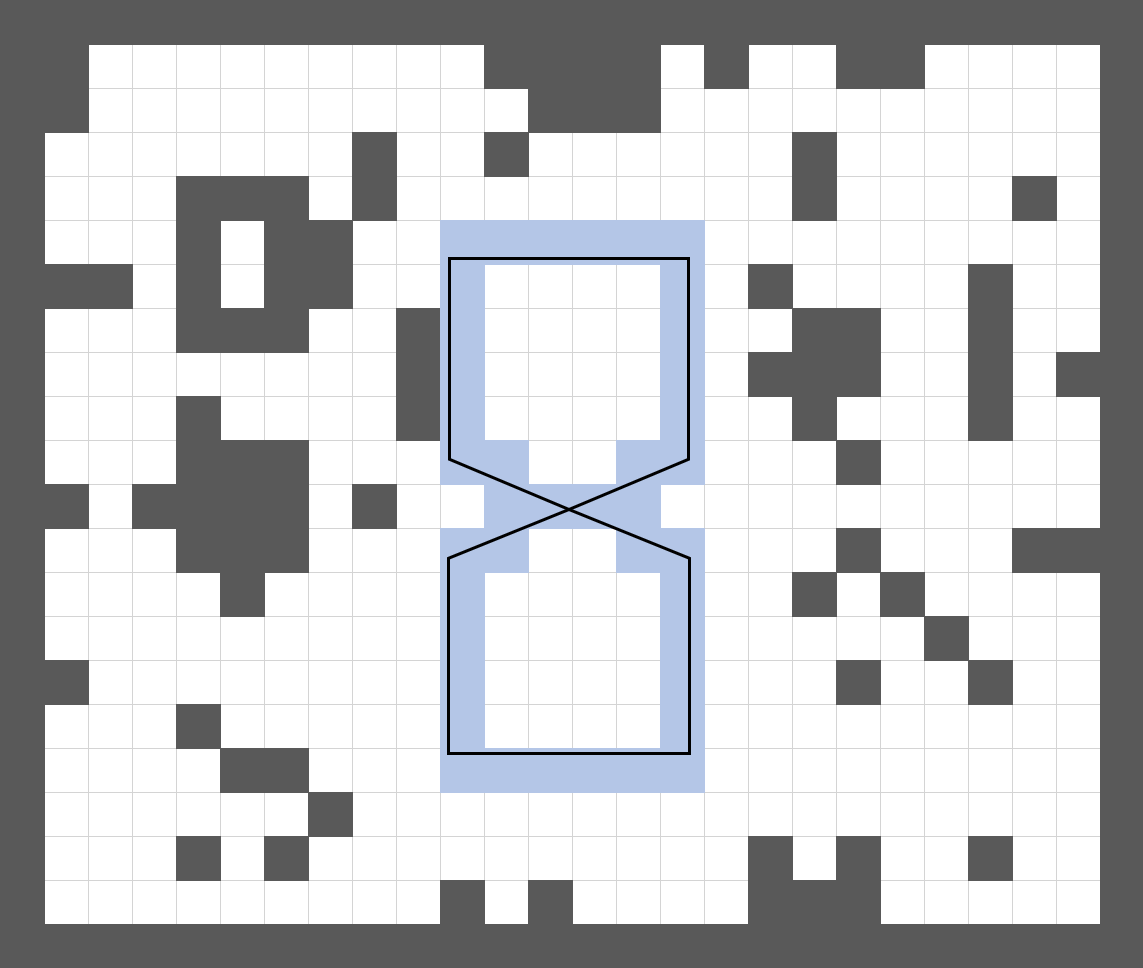
\includegraphics[width=0.8\textwidth]{bresham_free.png}
			\caption{breshamfree}
			\label{fig:bresham_free}
		\end{figure}
		
		\begin{figure}[!ht]
			\centering
			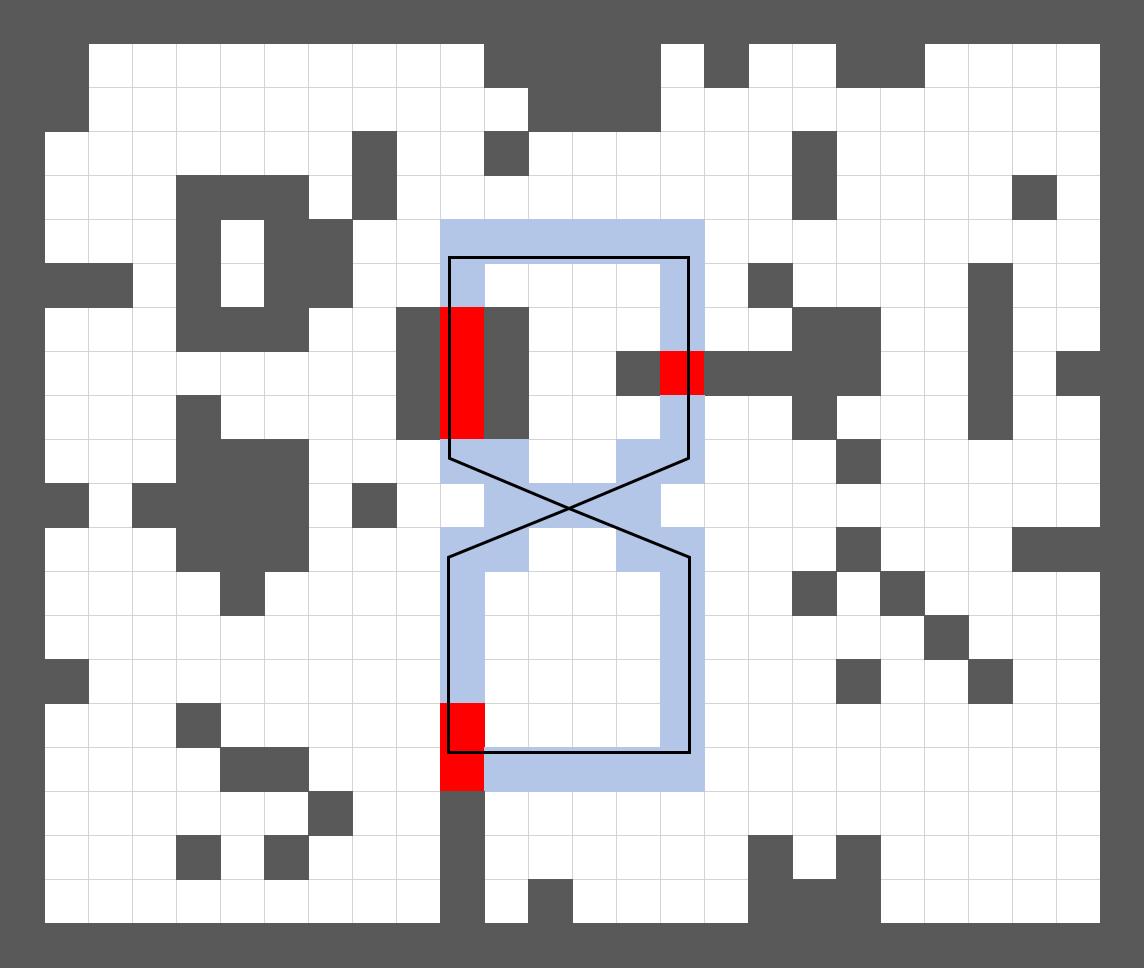
\includegraphics[width=0.8\textwidth]{bresham_colli.png}
			\caption{breshamcolli}
			\label{fig:bresham_colli}
		\end{figure}
	\section{基于NMPC和安全走廊的轨迹规划}
	在4.2节中我们针对铰接车对hybridAstar算法进行了改进,它将作为我们轨迹规划的热启动算法。本节中将介绍如何构建一个基于NMPC的轨迹规划算法,这是一个典型的OCP最优控制框架。
		\subsection{NMPC问题构建}
		铰接式车辆运动规划的最优控制问题可以表示为其一般形式,包括成本函数以及多个等式或不等式约束。与典型的优化问题不同,基于最优控制的轨迹规划还受到一组动态微分方程的约束。一般能耗和时间最优的代价函数定义如下:
		\begin{equation}
			\begin{aligned}
				J(x(t),u(t)) &= \int_{t_0}^{t_f}
				\left\| u(t)\right\|^2dt +w_t*\left\|t_f-t_0\right\|^2,    \\
				\left\|u(t)\right\|^2&=w_{uj}*\left\|jerk(t)\right\|^2+w_{uw}*\left\|\omega\right\|^2.
			\end{aligned} 
		\end{equation}
		其中 $w_t$、$w_{uj}$ 和 $w_{uw}$ 分别为时间代价权重、舒适度代价权重和铰接角能耗代价权重。$\left\|u(t)\right\|^2$ 用作输入能量消耗的度量,而 $\|t_f- t_0\|^2$ 确保时间持续时间的最优性,其中 $t_f$ 和 $t_0$ 分别为结束时间和开始时间。然后这个轨迹优化问题表示为:
		\begin{equation}
			\begin{aligned}
				&\left[x^*(t),u^*(t)\right] = minimize\ J(x(t),u(t)),\\      
				&s.t.\ \dot x(t)-f(x(t),u(t))=0,\\
				&x_l \leq x(t) \leq x_u, u_l \leq u(t) \leq u_u,t\in \left[0,t_f\right],\\
				&x(t_0)=x_{start},x(t_f)=x_{goal}.\label{4}
			\end{aligned}   
		\end{equation}
		在公式【】的约束中,$\dot x(t)-f(x(t),u(t))=0$表示运动方程约束,保证优化问题中轨迹的平滑性。变量$x_l$和$x_u$表示状态变量的下界和上界,$u_l$和$u_u$表示控制变量的下界和上界。此外,$x_{start}$和$x_{goal}$分别对应规划问题的起点状态和终点状态。对于如上NMPC形式的最优控制问题,处于问题的复杂度,我们并不在连续空间下进行求解。我们将它的状态方程进行离散化,求解它的最有离散子序列,即演变成一个NLP(Nonlinear Programming)问题。我们定义如下形式的解向量形式:
		\begin{equation}
			\begin{aligned}
				\xi &=\left[ \xi _{x}^{T},\xi _{y}^{T},\xi _{\theta}^{T},\xi _{\gamma}^{T},\xi _{v}^{T},\xi _{a}^{T},\xi _{\omega}^{T},\xi_{{jerk}}^{T},\xi _{\Delta t}^{T} \right] ^T,\\
				\xi _x&=\left[ x\left( 1 \right) ,...,x\left( N-2 \right) \right] ^T,\\
				\xi _{\omega}&=\left[ \omega \left( 0 \right) ,...,\omega \left( N-2 \right) \right] ^T.
			\end{aligned}   
		\end{equation}
		对于轨迹上的$N$个点,起点$P_0$和终点$P_{N-1}$是已知的。$\xi _{x}$的维度为$n=N-2$,$\xi _{y},\xi _{\theta},\xi _{\gamma},\xi _{v},\xi _{a}$一样。$\xi _{\omega}$的维度为$m=N-1$,$\xi_{jerk},\xi _{\Delta t}$一样。

		以上所构建的优化问题中所受到的约束有状态方程约束、状态受限、输入受限、起点约束和终点约束,并没有包含避障约束。沿用安全走廊的方法,和【3.3】一样,避障约束是不等式的形式。我们假设$g_f$为铰接车前桥的不等式约束函数,$g_r$为铰接车后桥的不等式约束函数。则最终的轨迹规划问题可以表示为:
		\begin{equation}
			\begin{aligned}
			&J\left( \xi \right) =w_{uj}*\lVert \xi _{jerk} \rVert _{2}^{2}+w_{uw}*\lVert \xi _{\omega} \rVert _{2}^{2}+w_t*I_{N-1}^{T}\xi _{\Delta t},\\
			s.t.\ \ &g_{kin}\left( k \right) =0,1\leq k\leq N-1,\\
			&g_f\left( k \right) <0,\,\,g_r\left( k \right) <0,1\leq k\leq N-2,\\
			&\hat{\xi}_{min}\le \hat{\xi}\le \hat{\xi}_{max},\xi _{\Delta tmin}<\xi _{\Delta t}<\xi _{\Delta tmax}.
			\end{aligned}   
		\end{equation}
		其中$\hat{\xi}=\left[ \xi _{\gamma}^{T},\xi _{v}^{T},\xi _{a}^{T},\xi _{\omega}^{T},\xi _{\text{jerk}}^{T} \right] ^T$,$g_{kin}$是状态方程约束。方程约束中未提到的变量都是无约束变量。

		\subsection{运动学约束}
		如公式,在第二章中我们介绍了铰接车的运动学模型。这个运动学模型的状态量为x,y,theta,gamma,受到微分方程的约束这些变量是天然连续的。系统的输入为速度v和铰接角速度omega,他们并没有受到微分方程的约束,这意味着v和omega在优化过程中直接作为优化变量是会突变的。这对于下层控制来说是不利的。为了解决这个问题,我们为系统引入高阶信息的连续性,假设系统的输入为jerk(加加速度或者舒适度)和omega。模型可以进一步写为:
		\begin{equation}
			\begin{aligned}
				\dot{x}=f( x,u ) \Longrightarrow \frac{d}{dt}\left[ \begin{array}{c}
					x_f\\
					y_f\\
					\theta\\
					\gamma\\
					v\\
					a\\
				\end{array} \right] =\left[ \begin{array}{c}
					vcos\theta\\
					vsin\theta\\
					vtan( \gamma /2 ) /L+\omega / (cos\gamma +1 )\\
					\omega\\
					a\\
					jerk\\
				\end{array} \right] 
			\end{aligned}   
		\end{equation}
		在这里 $x=\left[ x_f,y_f,\theta,\gamma,v,a \right]^T$ 为状态向量,分别表示前轴中点位置、航向角、铰接角、速度、加速度。输入向量由 $u=\left[jerk,w\right]^T$ 给出,其中 $jerk$ 为前轴中点加加速度(舒适度),$w$ 为铰接角速度。
		对于上述运动学方程我们对其进行离散化,采用一阶离散运动学模型,可表示为:
		\begin{equation}
			\begin{aligned}
				x( k ) =x( k-1 ) +\Delta t( k-1 ) f( x( k-1 ) ,u( k-1 ) ) 
			\end{aligned}   
		\end{equation}
		我们令 \(g_{\text{kin}} = [g_x^T\ g_y^T\ g_\theta^T\ g_\gamma^T\ g_v^T\ g_a^T]^T\),其中每个 \(g\) 对应 \(m = N-1\) 个等式约束。例如:
		\begin{equation}
			\begin{aligned}
				g_{x_f}( 0 ) =x_f( 1 ) -x_{start}-\Delta t( 0 ) \cdot v( 0 ) \cos \theta( 0 ) ,\\
				g_{x_f}( 1 ) =x_f( 2 ) -x_f( 1 ) -\Delta t( 1 ) \cdot v( 1 ) \cos \theta ( 1 ) ,\\
				...\\
				g_{y_f}( 0 ) =y_f( 1 ) -x_{start}-\Delta t( 0 ) \cdot v( 0 ) \sin \theta ( 0 ) ,\\
				g_{y_f}( 1 ) =y_f( 2 ) -y_f( 1 ) -\Delta t( 1 ) \cdot v( 1 ) \sin \theta ( 1 ) ,\\
				...
			\end{aligned}   
		\end{equation}
		使用惩罚函数将运动学约束纳入成本函数,表达式如下:
		\begin{equation}
			\mathcal{G}_{kin} = w_{kin}*\left \| g_{kin} \right \|_2^2
		\end{equation}
		梯度为:
		\begin{equation}
			\frac{\partial\mathcal{G}_{kin}}{\partial\xi}=2w_{kin}\cdot\frac{\partial g_{kin}^T}{\partial\xi}\cdot g_{kin}\label{18}
		\end{equation}
		其中 \(\frac{\partial g_{\text{kin}}^T}{\partial \xi}\) 表示所有运动约束向量的雅可比矩阵。假设第 \(i\) 类运动约束关于第 \(j\) 类变量的雅可比矩阵由 \(\psi_{ij} = \frac{\partial g^T_{i}}{\partial \xi_j}\) 给出。我们可以推出:
		\begin{equation}
			\begin{array}{c}
				\frac{\partial g_{k i n}^{T}}{\partial \xi}= \\
				{\left[\begin{array}{cccccc}
						\psi_{E} & 0 & 0 & 0 & 0 & 0 \\
						0 & \psi_{E} & 0 & 0 & 0 & 0 \\
						-\psi_{x \theta} & -\psi_{y \theta} & \psi_{E} & 0 & 0 & 0 \\
						0 & 0 & -\psi_{\theta \gamma} & \psi_{E} & 0 & 0 \\
						-\psi_{x v} & -\psi_{y v} & -\psi_{\theta v} & 0 & \psi_{E} & 0 \\
						0 & 0 & 0 & 0 & -\psi_{v a} & \psi_{E} \\
						0 & 0 & -\psi_{\theta \omega} & -\psi_{\gamma \omega} & 0 & 0 \\
						0 & 0 & 0 & 0 & 0 & -\psi_{\text {ajerk }} \\
						-\psi_{x \Delta t} & -\psi_{y \Delta t} & -\psi_{\theta \Delta t} & -\psi_{\gamma \Delta t} & -\psi_{v \Delta t} & -\psi_{a \Delta t}
					\end{array}\right]}
			\end{array}
		\end{equation}
		其中 $\psi _ = [_{n \times n}, 0_n] - [0_n, E_{n \times n}]$,其中 $E$ 为单位矩阵,且\(\psi_{ij} = \frac{\partial g^T_{i}}{\partial \xi_j}\)。
		\subsection{安全走廊的防碰撞约束处理}
		在本节中,我们将探讨避障约束在笛卡尔坐标系中的表述方法。我们仍然采用安全走廊模型对铰接车的避障进行全维建模,安全走廊的构建方法参照第3.3节中的全局规划方案。与全局规划中的处理方式不同,本节中我们将对车体结构进行建模。在全局规划中,车体被简化为质点模型,且车体结构的影响通过膨胀层来近似替代,这种方法虽然较为粗略,但其主要目的是快速生成一条长远的路径,以为局部规划提供导航指引。而局部规划则负责生成更加精细化的轨迹。

		首先,在平面上沿前端粗解生成一系列凸多边形,这些凸多边形依次相交形成安全走廊,所有优化轨迹点都将被约束在该走廊内。安全走廊如图3所示。
		\begin{figure}[!ht]
			\centering
			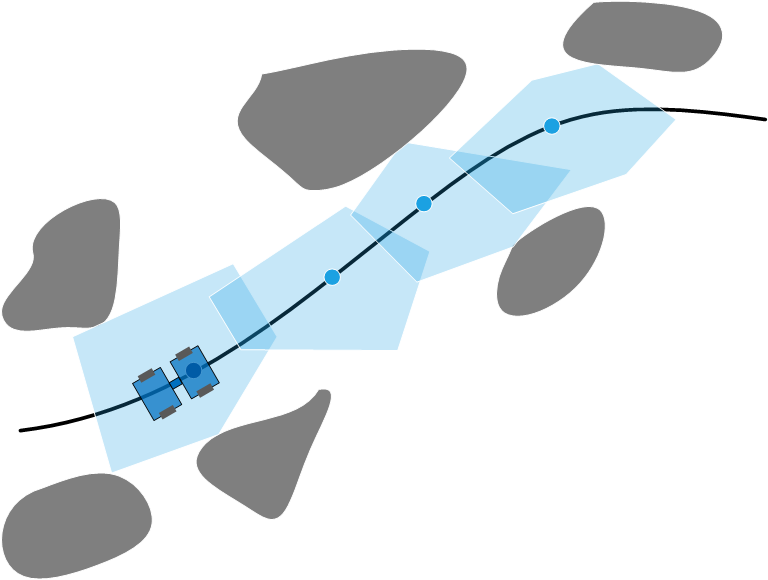
\includegraphics[width=0.8\textwidth]{安全走廊.png}
			\caption{安全走廊}
			\label{fig:安全走廊}
		\end{figure}
		根据凸集的性质,如果车辆的所有顶点都在凸包内,那么整个车辆就一定在凸包内。我们把铰接车前桥和后桥共八个顶点全部带入不等式【】,可以得到如下安全约束:
		\begin{equation}
			\left\{ \begin{matrix}
				A\left( R_{\theta}l_f+\sigma \right) -b<0,&		f=A,B,C,D\\
				A\left( R_{\gamma}R_{\theta}l_r+R_{\theta}l_{O_1}+\sigma \right) -b<0,&		r=E,F,G,H\\
			\end{matrix} \right. .
		\end{equation}.
		需要注意的是,所有顶点不一定都需要参与到避障约束中。由于铰接角的运动范围有限,仅利用前轴的四个顶点很多时候就足以实现有效的避障。
		为了方便表达,我们令
		\begin{equation}
			\begin{aligned}
			g_f\left( \sigma ,\theta ,\gamma \right) &=A\left( R_{\theta}l_f+\sigma \right) -b\\
			g_b\left( \sigma ,\theta ,\gamma \right) &=A\left( R_{\gamma}R_{\theta}l_r+R_{\theta}l_{O_1}+\sigma \right) -b.
			\end{aligned}
		\end{equation}
		这里$R_{\theta +\gamma}=R_{\theta}R_{\gamma},\ R_{\theta}=\left[ \begin{matrix}
			cos\theta&		-sin\theta\\
			sin\theta&		cos\theta\\
		\end{matrix} \right] $。
		路径上第$k$个点处的走廊约束关于$\sigma_k,\theta_k$和$\gamma_k$的梯度由下式给出:
		\begin{equation}
			\begin{aligned}
			\frac{\partial g_{f}^{T}(k)}{\partial \sigma _k}&=A_{k}^{T},\frac{\partial g_{f}^{T}(k)}{\partial \gamma _k}=0,\frac{\partial g_{f}^{T}(k)}{\partial \theta _k}=l_{f}^{T}\frac{\partial R_{\theta}^{T}}{\partial \theta _k}A_{k}^{T},\\
			\frac{\partial g_{r}^{T}(k)}{\partial \sigma _k}&=A_{k}^{T},\frac{\partial g_{r}^{T}(k)}{\partial \gamma _k}=l_{r}^{T}\frac{\partial R_{\theta +\gamma}^{T}}{\partial \gamma _k}A_{k}^{T},\\
			\frac{\partial g_{r}^{T}(k)}{\partial \theta _k}&=l_{r}^{T}\frac{\partial R_{\theta +\gamma}^{T}}{\partial \theta _k}A_{k}^{T}+l_{o1}^{T}\frac{\partial R_{\theta}^{T}}{\partial \theta _k}A_{k}^{T}.
			\end{aligned}
		\end{equation}

		对于上述走廊的不等式约束,我们使用罚函数将约束加入到代价函数中。罚函数依旧使用公式【】。为了方便表达,我们定义 \([]\) 为逐元素运算符,例如 \([\cdot]\) 表示逐元素乘法,\(S[x]\) 表示对$x$的所有元素进行函数 \(S\)运算 。得到以下结果,其表达为:
		\begin{equation}
			\mathcal{G}_c =\mathcal{G}_{f}+\mathcal{G}_{r}=w_{c}\cdot \sum_{k=1}^{N-2}\sum_{i=0}^{d-1}(S[g_f(k)] + S[g_r(k)]).\label{20}
		\end{equation}
		其中$d$为矩阵$A_k$的行数。为了确保连续可微性,松弛函数$S(x)$仍然使用第三章中的公式(3-21)。对【上式】中的各项分别进行求导得到走廊的惩罚项的梯度:
		\begin{equation}
			\begin{aligned}
				\frac{\partial \mathcal{G}_{f,r}}{\sigma \left( k \right)}&=\sum_{i=0}^{d-1}{A}_{k}^{T}S^{'}\left[ g_{f,r}\left( k \right) \right] =A_{k}^{T}S^{'}\left[ g_{f,r}\left( k \right) \right] I_d,\\
				\frac{\partial \mathcal{G}_f}{\xi _{\theta}\left( k \right)}&=l_{f}^{T}\frac{\partial R_{\theta}^{T}\left( k \right)}{\partial \theta \left( k \right)}A_{k}^{T}S^{'}\left[ g_f\left( k \right) \right] I_d,\\
				\frac{\partial \mathcal{G}_r}{\xi _{\gamma}\left( k \right)}&=l_{r}^{T}\frac{\partial R_{\theta +\gamma}^{T}\left( k \right)}{\partial \gamma \left( k \right)}A_{k}^{T}S^{'},\\
				\frac{\partial \mathcal{G}_r}{\xi _{\theta}\left( k \right)}&=\left( l_{r}^{T}\frac{\partial R_{\theta +\gamma}^{T}\left( k \right)}{\partial \theta \left( k \right)}+l_{o1}^{T}\frac{\partial R_{\theta}^{T}\left( k \right)}{\partial \theta \left( k \right)} \right) A_{k}^{T}S^{'}\left[ g_r\left( k \right) \right] I_d,\\
				\sigma \left( k \right) &=\left[ \xi _x\left( k \right) ,\xi _y\left( k \right) \right] ^T.\left[ g_r\left( k \right) \right] I_d
			\end{aligned}
		\end{equation}
		
		\subsection{变量的边界约束}
		在实际的系统中,系统的输入和状态往往不是无边界的,例如铰接车的速度、加速度、加加速度、铰接角等变量,所以我们要对这些变量进行约束分析。由于边界约束同样和走廊约束一样是不等式约束,所以我们仍然采用走廊约束处理方法,使用松弛函数$S(\cdot)$加入到代价函数中。为方便起见,我们省略了下标,变量边界约束对应的罚函数项和其梯度如下:
		\begin{equation}
			\begin{aligned}
				\mathcal{G}_b&=w_b\cdot \sum_{k=0}^{cols}{\left( S\left[ \hat{\xi}_{min}-\hat{\xi} \right] +S\left[ \hat{\xi}-\hat{\xi}_{max} \right] \right)}\\
				&=w_b\cdot I_{N-2}^{T}\left( S\left[ \hat{\xi}_{min}-\hat{\xi} \right] +S\left[ \hat{\xi}-\hat{\xi}_{max} \right] \right)\\
				\frac{\partial \mathcal{G}_b}{\hat{\xi}}&=w_b\cdot \left( S^{'}\left[ \hat{\xi}-\hat{\xi}_{max} \right] -S^{'}\left[ \hat{\xi}_{min}-\hat{\xi} \right] \right)
			\end{aligned}
		\end{equation}

		\subsection{时间正则化约束}
		在我们的轨迹优化问题中,每两个轨迹点之间的时间$\Delta t$是灵活变化且独立的,纳入了优化变量当中。它同样和走廊约束一样属于不等式约束,与之不同的是,时间项$\Delta t$必须严格大于0,这是硬约束。使用松弛函数对时间项进行惩罚属于约束软化的过程,在极端的场景下仍然可能出现$\Delta t \ge 0$,即使在下一步数值迭代过程中$\Delta t$又回到小于0。但是中间出现$\Delta t \ge 0$这是反只觉得,不符合物理的规律。所以避免这种情况,我们不能使用松弛函数处理时间正则化约束。
		为了解决以上问题,我们使用一个sigmoid变换将$\Delta t$的取值范围区间映射到映射到 负无穷到正无穷,变换后的变量记为$\tau$。这个变换是微分同胚的,微分同胚变换前后不会为优化问题引入额外的极小值【】。
		\begin{equation}
			\begin{aligned}
				\Delta t\left( \tau \right) =\frac{\Delta t_{max}}{1+e^{-\frac{\tau}{\Delta t_{max}}}},\,\,\,\,\Delta t^{'}\left( \tau \right) =\frac{e^{-\frac{\tau}{\Delta t_{max}}}}{\left( 1+e^{-\frac{\tau}{\Delta t_{max}}} \right) ^2}
			\end{aligned}
		\end{equation}
		这里$-\infty <\tau <+\infty $,$0<\Delta t<\Delta t_{max}$。
		
		\subsection{迭代求解框架}
		在上面几个小节,利用惩罚函数来表示成本函数中的运动学约束,并使用松弛函数来表示成本函数中的走廊约束,对于时间正则化,我们将时间变量的取值范围转换为整个实数轴。
		由于时间变量发生了转换,我们不妨重新表示以下优化变量。令最终的优化变量$\eta =\left[ \xi _{x}^{T},\xi _{y}^{T},\xi _{\theta}^{T},\xi _{\gamma}^{T},\xi _{v}^{T},\xi _{a}^{T},\xi _{\omega}^{T},\xi _{\text{jerk}}^{T},\xi _{\tau}^{T} \right] ^T$,在这里$\xi _{\tau}$和最初优化变量$\xi$中的$\xi _{t}$是微分同胚的。于是代价函数可以重新写为:
		\begin{equation}
			\begin{aligned}
				\mathcal{J}\left( \eta \right) =J\left( \xi \right) +\mathcal{G}_{kin}+\mathcal{G}_c+\mathcal{G}_b
			\end{aligned}
		\end{equation}
		对应的梯度为
		\begin{equation}
			\begin{aligned}
				\frac{\partial \mathcal{J}}{\partial \xi _{jerk,\omega}}=2w_{uj,uw}\cdot \xi _{jerk,\omega},\frac{\partial \mathcal{J}}{\partial \xi _{\tau}}=\Delta t\left[ \xi _{\tau} \right]
			\end{aligned}
		\end{equation}
		在等式约束部分【】,我们推导出了运动学约束的雅可比矩阵。现在,我们同样也要把对时间变量的导数部分进行替换,替换为
		\begin{equation}
			\begin{aligned}
				\psi _{i\tau}=\frac{\partial g_{i}^{T}}{\partial \xi _{\tau}}=\frac{\partial g_{i}^{T}}{\partial \xi _{\Delta t}}\cdot \Delta t\left[ \xi _{\tau} \right] 
			\end{aligned}
		\end{equation}
		其中$\mathcal{G}_{\text{kin}},\mathcal{G}_c,\mathcal{G}_b$由【】【】【】提供。

	\section{本章小结}
	在本章中,我们提出了一种基于安全走廊的无人铰接车局部轨迹规划方法,并通过最优控制框架对其进行建模与求解。首先,我们对铰接车的外观进行了通用性的建模,并通过简化车辆形状为两个矩形的连接,转化了避障问题为几何碰撞问题。其次,提出了针对铰接车的Hybrid A*算法改进,通过调整节点拓展策略并结合铰接车的运动学特性,优化了路径规划的效率与准确性。我们还设计了适用于铰接车的碰撞检测算法,利用栅格地图与Bresenham算法进行高效的障碍物检测。

	在轨迹优化方面,我们构建了基于非线性模型预测控制(NMPC)的轨迹规划方法,定义了优化问题并加入了动力学约束、运动学约束及避障约束。通过引入适合铰接车的运动学模型和代价函数,确保了在求解过程中能够考虑车辆的舒适度与能效,同时解决了车辆输入突变的问题。

	通过本章的研究,我们不仅改进了传统轨迹规划算法以适应铰接车的特殊运动特性,还设计了高效的碰撞检测与轨迹优化方案,为无人铰接车在复杂环境中的局部路径规划提供了有效的解决方案。
	
	\chapter{无人铰接车运动规划系统仿真实验}
	\section{系统集成}
		\subsection{仿真环境介绍}
		\subsection{自主导航系统框架介绍}
	\section{长远距离自主避障实验}
	\section{自主泊车和侧方位停车实验}
	\section{本章总结}

	\reference{ref.bib}

	\customizedappendix{
		\begin{align}
			\theta&=\omega t\notag\\
			a&=\cos\theta \label{eq:appendix1_a}\\
			b&=\sin\theta \label{eq:appendix1_b}\\
			a^2+b^2&=1
			\label{eq:appendix1_a^2+b^2}
		\end{align}
		
		\begin{subequations}
			\label{eq2:appendix1_identity_a_b}
			\begin{align}
				\theta&=\omega t\notag\\
				a&=\cos\theta \label{eq2:appendix1_a}\\
				b&=\sin\theta \label{eq2:appendix1_b}\\
				a^2+b^2&=1
				\label{eq2:appendix1_a^2+b^2}
			\end{align}
		\end{subequations}
	}

	\customizedappendix{
		\begin{align}
			\theta&=\omega t\notag\\
			a&=\cos\theta \label{eq:appendix2_a}\\
			b&=\sin\theta \label{eq:appendix2_b}\\
			a^2+b^2&=1
			\label{eq:appendix2_a^2+b^2}
		\end{align}
		
		\begin{subequations}
			\label{eq2:appendix2_identity_a_b}
			\begin{align}
				\theta&=\omega t\notag\\
				a&=\cos\theta \label{eq2:appendix2_a}\\
				b&=\sin\theta \label{eq2:appendix2_b}\\
				a^2+b^2&=1
				\label{eq2:appendix2_a^2+b^2}
			\end{align}
		\end{subequations}
	}


	\achievement{
		{\vspace{-0.1em}\noindent\textbf{\songtib\zihao{-4} 1.\enspace 发表的学术论文}\vspace{-0.41em}}    % 无学术论文时此项不必列出
		\begin{enumerate}[leftmargin=1.52em,itemsep=-0.4em,label={[\arabic*]}]\zihao{5}%%%%%%% 这一行的设定不要修改!!!
			\item ×××, ×××. 并联2-RRR/UPRR踝关节康复机器人机构及其运动学[J]. 机器人, 2010, 32(1): 6-12. (EI收录号: 20101212786168)
			\item ×××, ×××. 空间并联机构连续刚度非线性映射研究[J]. 机械工程学报, 2008, 44(8): 20-25. (EI收录号: 083911606237)
			\item ×××, ×××. A sampling robot for high dust and strong corrosion environment[C]//International Conference on Robotic and Biomimetics, Tianjin, 2010: 828-832. (EI收录号: 20111313856140)
			\item ×××, ×××. 双重驱动四自由度并联机构型综合[J]. 机械设计与研究, 2008, 24(1): 51-53.
			\item $\cdots$要与参考文献格式一致!!!
		\end{enumerate}

		%%%%%%%%%%%%%%%%%%%%%%%%%%%%%%%%%%%%%%%%%%%%专著/译著
		{\vspace{-0.44em}\noindent\textbf{\songtib\zihao{-4} 2.\enspace 发表的专著/译著(无著作时此项不必列出)}\vspace{-0.41em}}    % 无专著/译著时此项不必列出
		\begin{enumerate}[leftmargin=1.52em,itemsep=-0.4em,label={[\arabic*]}]\zihao{5}%%%%%%% 这一行的设定不要修改!!!
			\item ×××, ×××. 高等空间机构学 [M]. 北京: 机械工业出版社, 2010.
			\item ×××, ×××. 空间并联机构导论 [M]. ×××, 译. 秦皇岛: 燕山大学出版社, 2020.
		\end{enumerate}

		%%%%%%%%%%%%%%%%%%%%%%%%%%%%%%%%%%%%%%%%%%%%%%%%%%%%%%%%%%%%%%%%%%%%%%%%%%%%%%%%%%%%%%
		{\vspace{-0.44em}\noindent\textbf{\songtib\zihao{-4} 3.\enspace 申请及已获得的专利(无专利时此项不必列出)}\vspace{-0.41em}}    % 无专利时此项不必列出
		\begin{enumerate}[leftmargin=1.52em,itemsep=-0.4em,label={[\arabic*]}]\zihao{5}%%%%%%% 这一行的设定不要修改!!!
			\item ×××, ×××. 具有远程运动中心的三自由度转动并联机构: 中国, 200910073844.8 [P]. 2011-01-05.
			\item ×××, ×××. 五自由度双重驱动并联机构: 中国, 200910075071.7 [P]. 2011-01-05.
		\end{enumerate}

		%%%%%%%%%%%%%%%%%%%%%%%%%%%%%%%%%%%%%%%%%%%%%%%%%%%%%%%%%%%%%%%%%%%%%%%%%%%%%%%%%%%%%%
		{\vspace{-0.44em}\noindent\textbf{\songtib\zihao{-4} 4.\enspace 科研获奖(无奖励时此项不必列出)}\vspace{-0.41em}}    % 无奖励时此项不必列出
		\begin{enumerate}[leftmargin=1.52em,itemsep=-0.4em,label={[\arabic*]}]\zihao{5}%%%%%%% 这一行的设定不要修改!!!
			\item ×××, ×××. 机器人机型综合及结构分析理论. XX省科学技术二等奖, 2009.
		\end{enumerate}
	}

	\acknowledgement{
	}
\end{document}
